\documentclass[12pt]{article}
\usepackage{geometry}
\geometry{a4paper}
\usepackage[utf8]{inputenc}
\usepackage{amsmath,amssymb}
\usepackage{hyperref} % verlinkungen
\usepackage{textcomp}
\usepackage{flafter}
\usepackage{booktabs}
\usepackage{array}
\usepackage{paralist}
\usepackage{dsfont} \usepackage{color}
\usepackage{bbold}
\usepackage{float}
\usepackage[font=scriptsize,labelfont=bf]{caption}
%\usepackage[font=footnotesize,labelfont=bf]{caption}
\usepackage{subcaption}
\usepackage{fancyhdr}
\setlength{\headheight}{15.2pt}
\pagestyle{fancy}
\usepackage{listings} 
\usepackage{pict2e}
\usepackage{xfrac}
\usepackage[english]{babel}
\usepackage{mathtools}
\usepackage{graphicx}



%%%%%%%%         EIGENEBEFEHLE  %%%%%%%%%
\newcommand{\ddt}{\frac{\partial}{\partial{t}}}
\newcommand{\dnach}[1]{\frac{\partial}{\partial{#1}}}
\newcommand{\ddnach}[2]{\frac{\partial{#1}}{\partial{#2}}}
\newcommand{\dddnach}[3]{\frac{\partial^2{#1}}{\partial{#2} \partial{#3}}}
\newcommand{\dznach}[2]{\frac{\partial^2{#1}}{\partial{#2}^2}}
\newcommand{\vnabla}{\mathbf{\nabla}}
\newcommand{\emathbf}[1]{\mathbf{\hat{#1}}}
\newcommand{\bra}[1]{\langle{#1}|}
\newcommand{\ket}[1]{|{#1}\rangle}
\newcommand{\bracket}[2]{\langle{#1}|{#2}\rangle}
\newcommand{\up}{\uparrow}
\newcommand{\down}{\downarrow}
\newcommand{\updown}{\uparrow\downarrow}
\newcommand{\downup}{\downarrow\uparrow}
\newcommand{\upup}{\uparrow\uparrow}
\newcommand{\downdown}{\downarrow\downarrow}
\newcommand{\sandwich}[2]{\bra{#1} #2 \ket{#1}}
\newcommand{\fsqrt}[2]{\sqrt{\frac{#1}{#2}}}
\newcommand{\GammaK}{{\Gamma_k}}

\definecolor{mygreen}{rgb}{0,0.6,0}
\definecolor{mygray}{rgb}{0.5,0.5,0.5}
\definecolor{mymauve}{rgb}{0.58,0,0.82}

\lstset{%
  backgroundcolor=\color{white},   % choose the background color; you must add \usepackage{color} or \usepackage{xcolor}
  basicstyle=\footnotesize,        % the size of the fonts that are used for the code
  breakatwhitespace=false,         % sets if automatic breaks should only happen at whitespace
  breaklines=true,                 % sets automatic line breaking
  captionpos=b,                    % sets the caption-position to bottom
  commentstyle=\color{mygreen},    % comment style
  %deletekeywords={...},            % if you want to delete keywords from the given language
  %escapeinside={\%*}{*)},          % if you want to add LaTeX within your code
  extendedchars=true,              % lets you use non-ASCII characters; for 8-bits encodings only, does not work with UTF-8
  frame=single,                    % adds a frame around the code
  keepspaces=true,                 % keeps spaces in text, useful for keeping indentation of code (possibly needs columns=flexible)
  keywordstyle=\color{blue},       % keyword style
  language=C,                 % the language of the code
  %morekeywords={*,...},            % if you want to add more keywords to the set
  numbers=left,                    % where to put the line-numbers; possible values are (none, left, right)
  numbersep=5pt,                   % how far the line-numbers are from the code
  numberstyle=\tiny\color{mygray}, % the style that is used for the line-numbers
  rulecolor=\color{black},         % if not set, the frame-color may be changed on line-breaks within not-black text (e.g. comments (green here))
  showspaces=false,                % show spaces everywhere adding particular underscores; it overrides 'showstringspaces'
  showstringspaces=false,          % underline spaces within strings only
  showtabs=false,                  % show tabs within strings adding particular underscores
  stepnumber=2,                    % the step between two line-numbers. If it's 1, each line will be numbered
  stringstyle=\color{mymauve},     % string literal style
  tabsize=2,                       % sets default tabsize to 2 spaces
  %title=\lstname                   % show the filename of files included with \lstinputlisting; also try caption instead of title
}

\lhead[\ ]{\ }
\chead[\ ]{\ }
\rhead[\ ]{\ }

\lfoot[\ ]{\ }
\cfoot[\ ]{\ }
\rfoot[\ ]{\ }

%%%%%%%%%%%%%%%%%%%%%%%%%%%%%%%%%%%%%%%%%%%%

\begin{document}
\title{Simulation of Nano Particles in a Laser Trap}
\author{Mathias H\"old, BSc.}
\date{2016}
\maketitle
\thispagestyle{empty}
\newpage
\section{Introduction}
%something about computer science in general, optical tweezers and the need to study the
%systems on computers yada yada





\newpage
\section{Motivation}
%introduction of the experiment, the problem and the idea
The starting point of this thesis is an experiment conducted by Gieseler et al \cite{Gieseler2014}. It is an optical tweezer experiment, where the
motion of a glass nanoparticle in a laser trap was used to investigate the fluctuation theorem\cite{Crooks1999}.
\subsection{Experimental setup}
In the experiment, a silica nano particle with a radius of about 75 nm and mass of about $3 \times 10^{-18}$kg is trapped in a laser beam within a
vacuum chamber. The trapping of the silica nano particle is achieved by a gradient force of the
laser beam acting on the particle. The experimental setup is depicted in Fig.~\ref{fig:setup}.\\
The particle fluctuates within the trap in all three spatial directions. These fluctuations can be approximated
such that they are decoupled, which means that they can be described by a one-dimensional Langevin equation:
\begin{equation}
    \label{eq:langevin}
    \ddot{x} + \Gamma_0 \dot{x} + \Omega^2_0x = \frac 1 m \left(F_\text{fluct} + F_\text{ext}\right)
\end{equation}
%The experiment is set up as follows: a glass sphere with radius $r \approx 75$ nm and mass $m \approx 3 \times 10^{-18}$ kg is trapped in a laser beam
%in a vacuum chamber. The initial state of the glass particle is prepared by modulation of the laser, such that the oscillation of the glass particle
%is suppressed in every direction. This is done by measuring the oscillation of the particle in every direction (assuming that the oscillation in every
%direction is decoupled) and using this information as feedback for the laser. This experimental setup can be seen in figure \ref{fig:setup}.
\begin{figure}[H]
    \begin{center}
        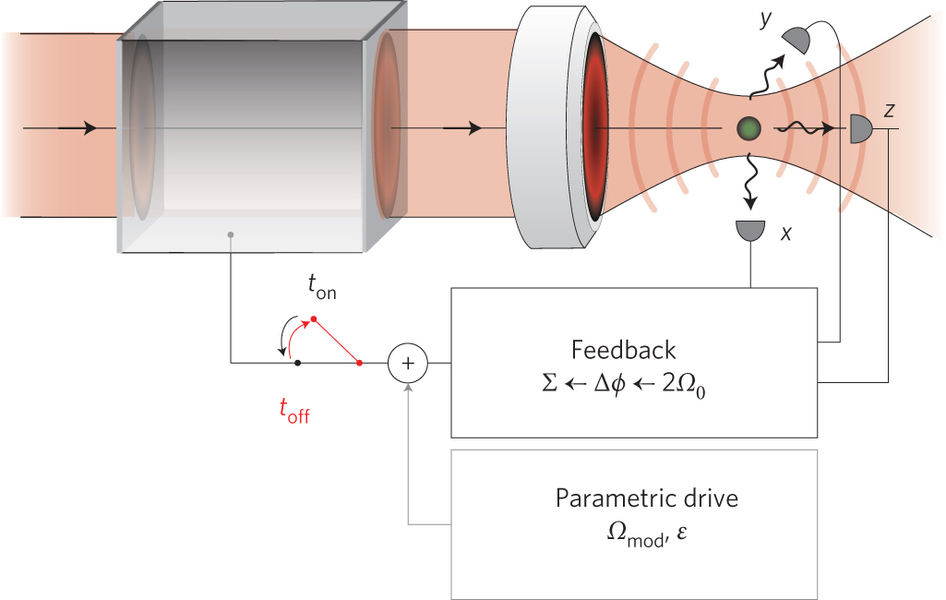
\includegraphics[scale=0.3]{images/experimental_setup.jpg}
        \caption{Experimental setup of the optical tweezer experiment. A silica nano particle is trapped in a laser beam via gradient force in a
        vacuum. The feedback is used to cool down the particle and create a non-equilibrium steady state. In the first part of the experiment, the
    feedback is turned off and the motion of the particle towards an equilibrated state is observed. In the second part of the experiment, the steady state
of the particle is modified by a parametric drive. Both the parametric drive and the feedback are turned off and -- as in the first part -- the
motion of the particle towards an equilibrated state is observerd. Figure taken from \cite{Gieseler2014}.}
        \label{fig:setup}
    \end{center}
\end{figure}
On the left hand side we have the position $x$ (and its derivatives $\dot{x}$, the velocity and $\ddot{x}$, the acceleration), the friction 
coefficient $\Gamma_0$ and the angular frequency $\Omega_0$ that describes the fluctuation along the chosen axis. On
the right hand side, there are two forces. The first one is $F_\text{fluct}$, which describes a stochastic force caused by interactions with the gas
in the vacuum chamber. This force is given by
\begin{equation}
    \label{eq:ffluct}
    F_\text{fluct} = \sqrt{2m\Gamma_0k_BT_0} \ \xi\left(t\right)
\end{equation}
where $T_0$ is the temperature of the heat bath (i.e., the surrounding gas in the vacuum chamber), $k_B$ is the Boltzmann constant and $\xi(t)$ is
white noise, which obeys the equations $\left\langle\xi(t)\right\rangle= 0$ and $\left\langle\xi(t)\xi(t')\right\rangle= \delta(t-t')$, which means
that it is a random force. The term $\Gamma_0$ appears in the formula \eqref{eq:ffluct} 
due to the fluctuation-dissipation theorem, which links the damping rate to the stochastic force.\\
%The external force $F_\text{ext}$ is part of the experimental setup, where the frequency of the fluctuation along an axis, $\Omega_0$, is measured and
%used to suppress the motion along said axis. This causes a decrease in the particle fluctuations and thus acts as a cooling mechanism for the particle
%in the trap. This process creates a non-equilibrium steady state $\rho_{ss}(u,\alpha)$, which is not known analytically. This state is the starting
%point of this thesis.\\
\subsection{Model of the Surrounding Gas}
J. Millen et al.~\cite{MillenJ.2014} worked on a similar experimental setup (without the feedback mechanism) and investigated the heating of the
particle in the trap as well as the gas surrounding the particle.\\
They start from the premise that there are 4 different temperatures one has to consider in such an experiment: the temperature of the gas particles
before interacting with the nano particle $T_\text{imp}$ (for \textit{impinging}), the temperature of the gas particles after 
interaction $T_\text{em}$ (for emerging), the surface temperature of the nano particle $T_\text{sur}$ and the temperature of the 
center of mass of the nano particle $T_\text{COM}$. The experimental setup
and the different temperatures are depicted in Fig.~\ref{fig:levitation}.\\
\begin{figure}[H]
    \begin{center}
        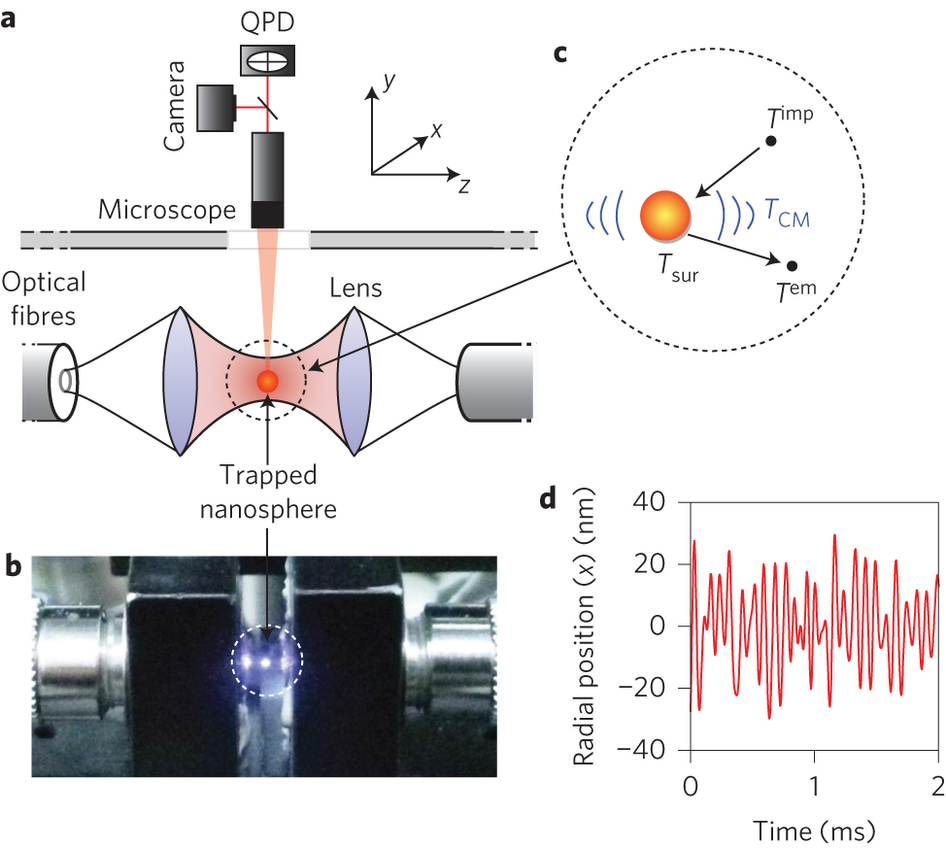
\includegraphics[scale=0.2]{images/nnano_millen.jpg}
        \caption{The experimental setup used by Millen et al. In \textbf{a} the experiment is schematically depicted and \textbf{b} shows a photograph
            of the actual experimental setup. In \textbf{c} the 4 different temperatures that are present during the experiment are depicted and
        \textbf{d} shows the position of the particle in the trap over time. The image was taken from~\cite{MillenJ.2014}}
        \label{fig:levitation}
    \end{center}
\end{figure}
Since the two temperatures of the gas, $T_\text{imp}$ and $T_\text{em}$, are not equal, the gas surrounding the nano particle is not in a thermal
equilibrium, which is in contrast to the assumption in many optical tweezer experiments. Since the gas particles only interact with the nano particle
in the trap and not wich each other, this situation creates two heat baths of different temperatures with the nano particle acting as a mediator
between those two baths. This situation is depicted in
Fig.~\ref{fig:heatbaths}.
\begin{figure}[H]
    \begin{center}
        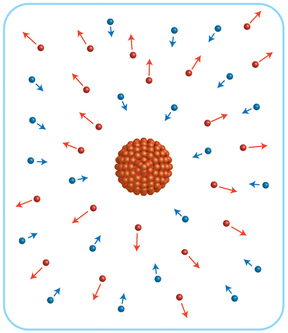
\includegraphics[scale=0.5]{images/nano_nonequilibrium_cropped.jpg}
        \caption{Schematic picture of the two heat baths. The (hot) nano particle interacts with the (cold) incoming gas particles and they leave with
        a higher temperature. The incoming and outgoing particles do not interact with each other and thus create two separate heat baths with
    different temperatures. Image modified from \cite{Kroy2014}}
        \label{fig:heatbaths}
    \end{center}
\end{figure}
The one dimensional Langevin equation \eqref{eq:langevin} has to be modeled to include the different friction coefficients of the two heat baths. The
model derived in \cite{MillenJ.2014} is described in the following equation:
\begin{equation}
    M\ddot{x}(t) + M\left(\Gamma^\text{imp}+\Gamma^\text{em}\right)\dot{x}(t) + M\omega^2x(t) =F^\text{imp}+F^\text{em}
\end{equation}
where $x$ is the position of the nano particle, $\dot{x}$ and $\ddot{x}$ are the velocity and the acceleration, respectively, $M$ is the mass,
$\omega$ is the trap frequency, $\Gamma^\text{imp}$ and $\Gamma^\text{em}$ are the damping constants for the 
impinging particles and the emerging particles, respectively and $F^\text{imp}$ and $F^\text{em}$ are the associated noise terms, 
which satisfy $\langle F^\text{imp}\rangle= \langle F^\text{em} \rangle = 0$ individually.\\
Miller et al. investigate the dependence of the emerging temperature $T_\text{em}$ on the intensity of the laser for different sized nano particles
and different pressures.\\

%These four temperatures introduced in the paper, together with the surrounding pressure and the intensity of the laser 
%The existence of the two temperatures of the gas implies that, contrary to the assumption in many of the experiments, the gas is not in a thermal
%equilibrium. The Langevin equation (like the one in \eqref{eq:langevin}) has to be modeled k





\newpage
\section{Simulation}
%simulation techniques and general concept of the simulation itself, used methods and so on 
The problem at hand can be studied on an atomic level with the use of computer simulation. There is a variety of methods for computer simulations
that are widely used, one of which being molecular dynamics (MD) simulations.\\ 
The goal is to simulate the experiment depicted in Fig.~\ref{fig:setup} as accurately as possible. To achieve this, the setup has to be broken down
into individual pieced that can be modeled by using existing methods. The nano particle will be approximated by a cube of particles, sitting on an FCC
lattice that interact via a Lennard-Jones potential. The laser will be broken down into its two main purposes, as it acts as a trapping device as well
as a heat source for the nano particle. Surrounding the nano particle will be a gas chamber, that acts as a thermostat in the simulation, that will be
modeled as a box surrounding the nano particle. This box is filled with gas particles that interact with the nano particle via a soft-sphere potential
and do not interact with one another.\\
The following section will give a brief overview of the concepts used to simulate every part of the experiment.


\subsection{Molecular Dynamics}
Molecular dynamics~\cite{Frenkel2001} simulations is a technique for simulating, as the name suggests, the dynamics of a classical many-body system. In this case,
classical means, that the trajectories of the individual particles are calculated using classical mechanics rather then quantum mechanics. For
relatively big atoms/molecules this is a very good approximation, whereas for systems consisting of hydrogen or helium the effects of quantum
mechanics cannot be neglected and other methods have to be used.\\
The dynamics of the system are obtained by solving Newton's equations of motion for every particle. 

\subsection{The Nano Particle}
The glass particle from the experiment will be modeled as a system of particles interacting via a Lennard-Jones pair potential, 
\begin{equation}
    \label{eq:lj}
    U(r) = 4\varepsilon\left[\left(\frac\sigma r\right)^{12} - \left(\frac\sigma r\right)^6\right]
\end{equation}
where $\varepsilon$ is the depth of the potential well (and thus its unit is energy) and $\sigma$ is the distance at which the potential is zero. 
The form of the potential and the relation to the parameters is depicted in Fig. \ref{fig:lj}.
\begin{figure}[h]
    \begin{center}
        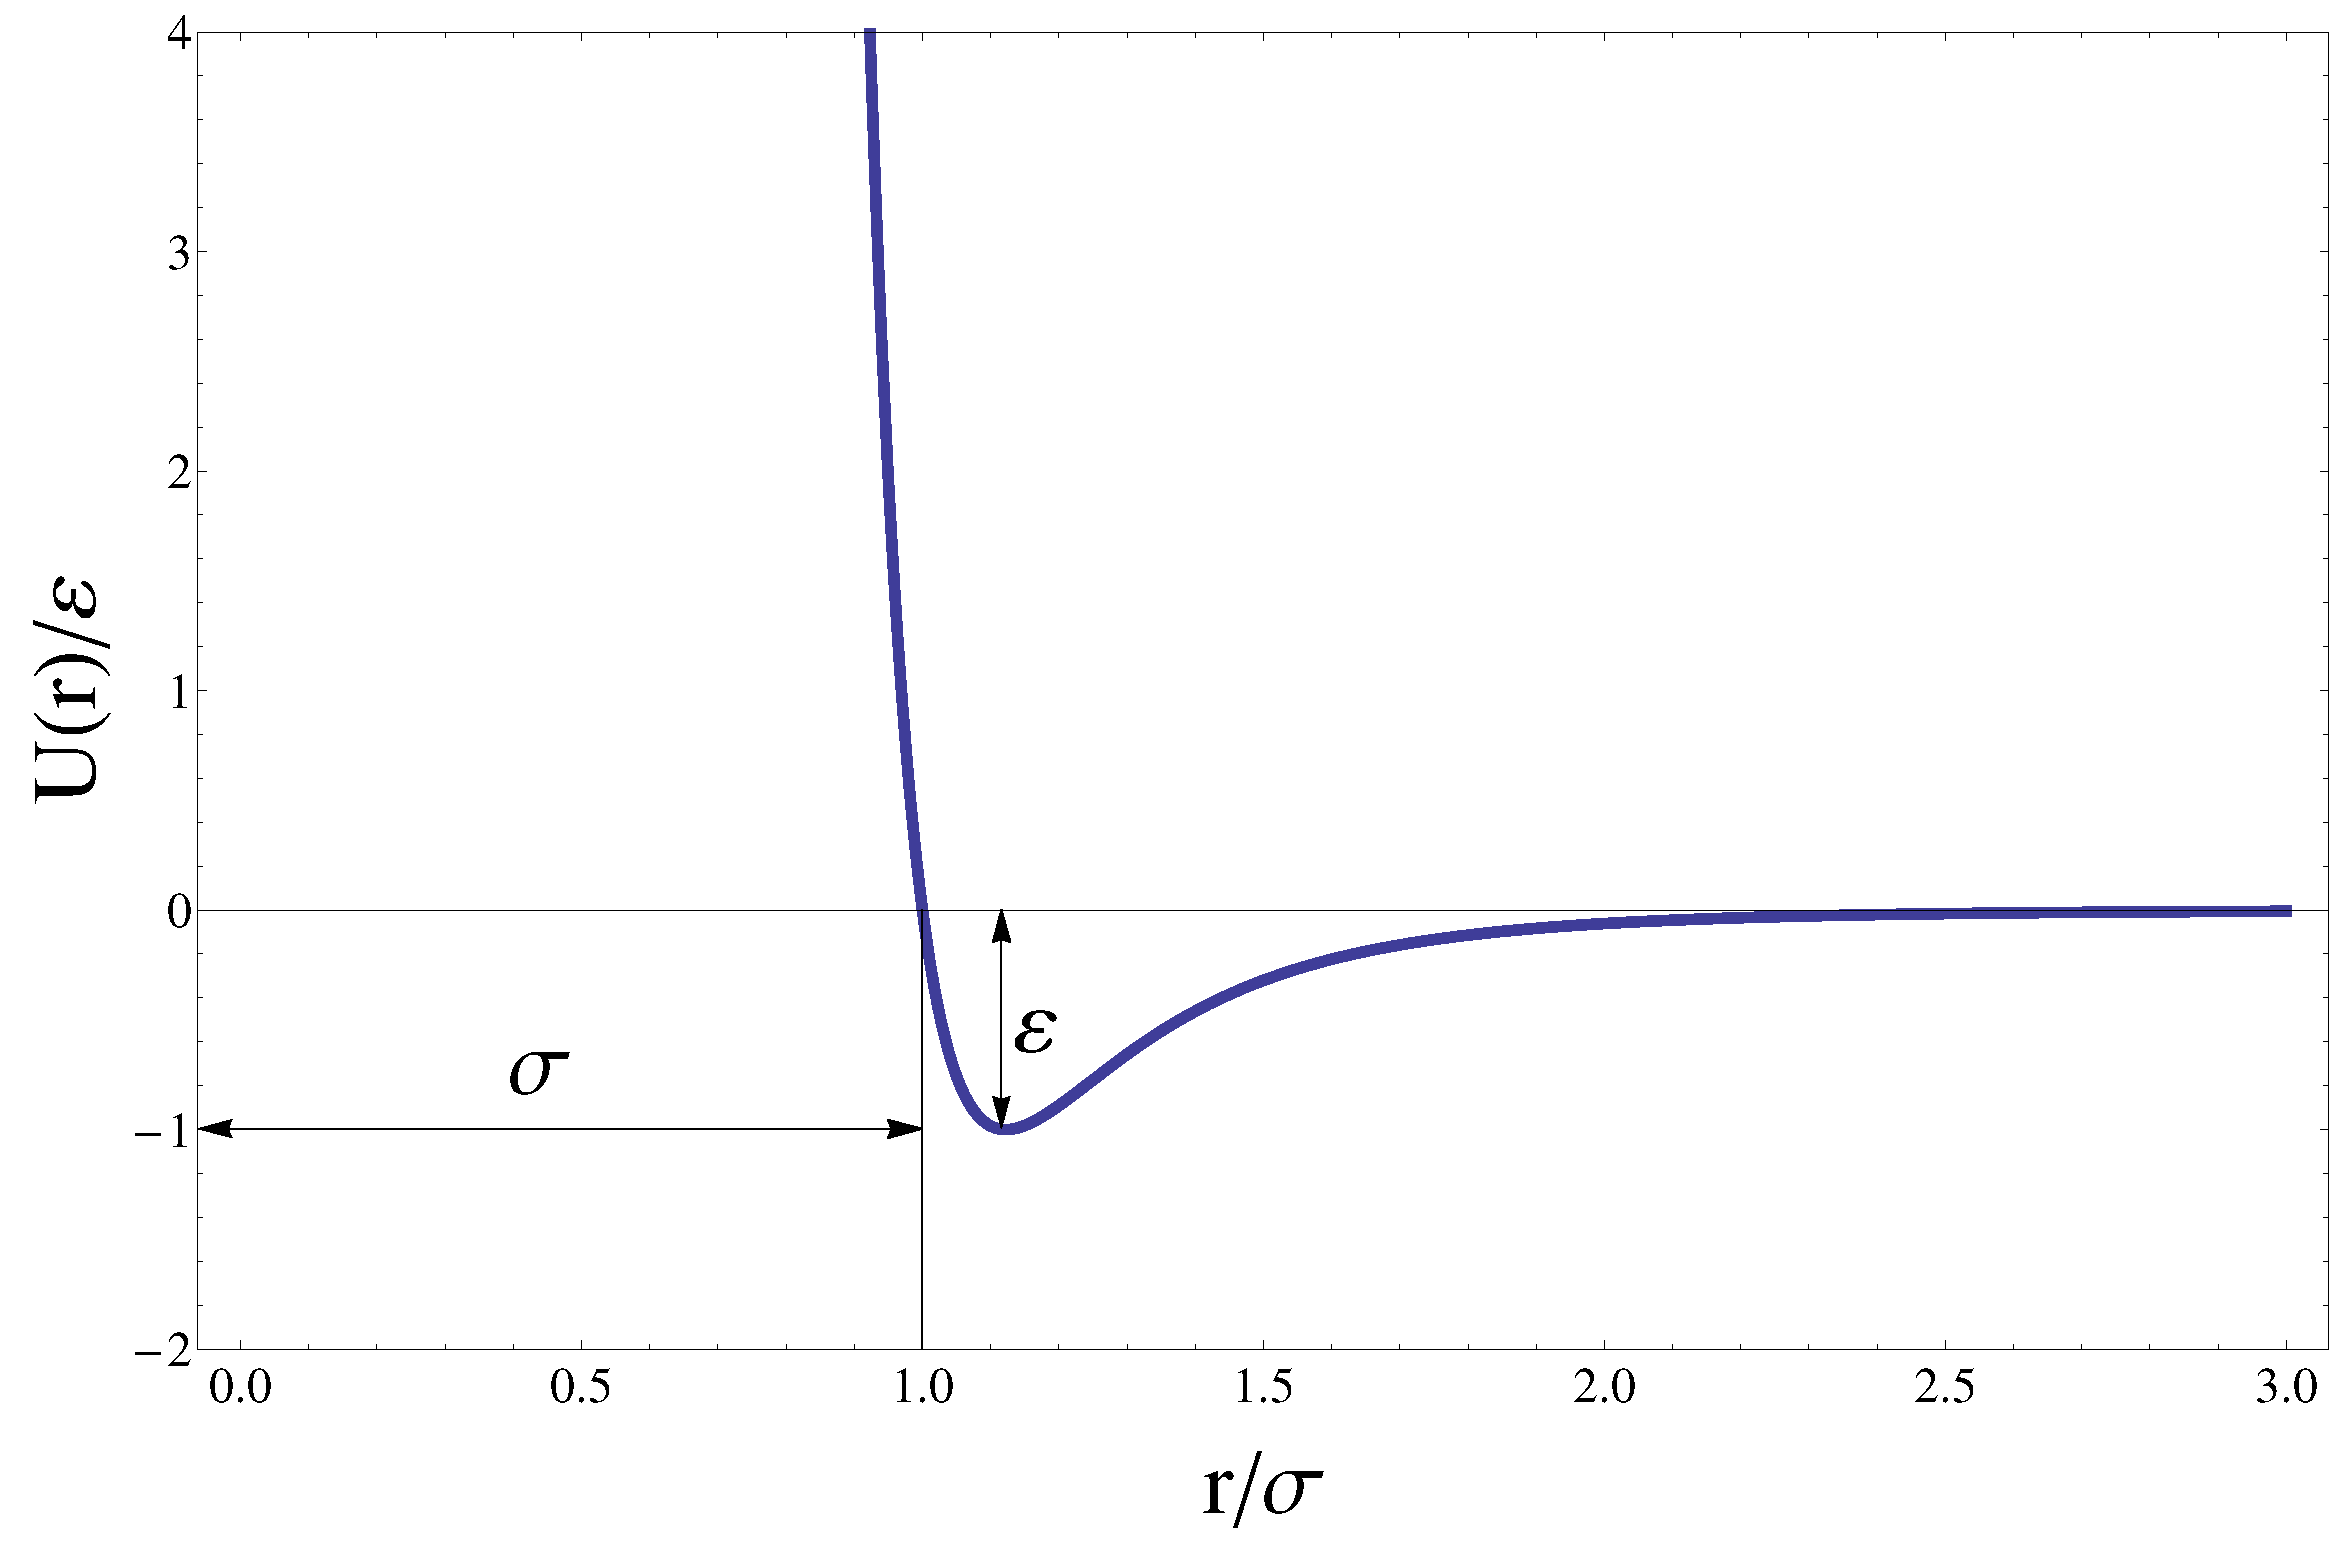
\includegraphics[scale=0.2]{images/LJ-2.pdf}
        \caption{The Lennard-Jones 12-6 potential from \eqref{eq:lj}. The x-axis is the particle distance divided by $\sigma$ and  the y-axis is the
        potential divided by the depth of the potential well.}
        \label{fig:lj}
    \end{center}
\end{figure}
Since $\varepsilon$ and $\sigma$ are crucial parameters for the simulation and do not change over time, it is practical to use them to
define the dimensions of the system. This means that the unit of distance is $\sigma$, the unit of energy is $\varepsilon$ and the unit of mass is 
the mass of the simulated particle. The so called \textit{reduced units} can be constructed from these three parameters and put into relation to the
original units. Here are some examples:
\begin{itemize}
    \item {distance:} $r^* = r/\sigma$
    \item {potential energy:} $U^* = U/\varepsilon$
    \item {temperature:} $T^* = k_B T/\varepsilon$
    \item {time:} $t^* = t\sqrt{\varepsilon/(m\sigma^2)}$
    \item {pressure:} $P^* = P\sigma^3/\varepsilon$
    \item {density:} $\rho^* = \rho \sigma^3$
\end{itemize}
One very popular choice for the simulated atoms is Argon because it is an inert gas and the atoms behave 
approximately like hard spheres which attract each other with weak van der Waals forces, which justifies the use of the Lennard-Jones potential. 
Argon has a mass of m = $6.69 \times 10^{-26}$ kg, $\sigma = 3.4 \times 10^{-10}$m and $\varepsilon = 1.65 \times 10^{-21}$J.\\
With the above introduced reduced units, the Lennard-Jones potential can be written as
\begin{equation}
    U(r^*) = 4\left[{r^*}^{-12} - {r^*}^{-6}\right].
\end{equation}
Since the reduced units will be used throughout the rest of this thesis, I will drop the asterisk henceforth.\\
From the Lennard-Jones potential the corresponding force can be calculated by taking the derivative with respect to the direction of interest:
\begin{eqnarray}
    F_{x} &=& -\frac{\partial}{\partial x} U(r) \nonumber\\
                &=& -\frac{\partial}{\partial x} 4\left[{r}^{-12} - {r}^{-6}\right] \nonumber\\
                &=& -4 \left[(-12){r}^{-13} - (-6){r}^{-7}\right] \frac{\partial r}{\partial x} \nonumber\\
                &=& 48 \left[r^{-13} - 0.5 \ r^{-7}\right] \frac{x}{r} \nonumber\\
    \label{eq:ljforce} &=& 48 \left[r^{-14} - 0.5 \ r^{-8}\right] x
\end{eqnarray}
The force in the y and z direction can be calculated analogously.\\
The initial configuration of the particles is a face centered cubic (FCC) lattice. A schematic of the FCC lattice is depicted in Fig. \ref{fig:fcc}.
With the choice of FCC as initial configuration, there are optimal numbers for the numbers of the particles in the system. Since once FCC cell 
shares its atoms with its next neighbours, the number of atom per unit cell is 4 -- 1/8 of a particle on eight corners and 1/2 of a particle on six faces.
The whole system of atoms is then created by repeating this cell structure. One convenient way is to arrange the unit cells in a cubic system, 
so if there are $M$ FCC unit cells on one edge, the whole system consists of $M^3$ cells. Since there are 4 particles per cell, 
there are ideal or so called \textit{magic numbers} for atoms for which this setup works perfectly: $N = 4M^3 = 4,32,108,256,500,864,\ldots$.\\
\begin{figure}[h]
    \begin{center}
        \begin{subfigure}[t]{0.4\textwidth}
            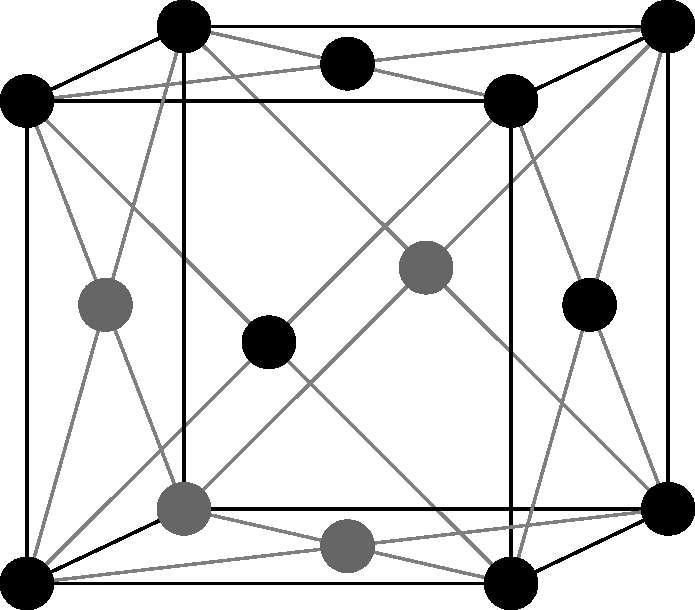
\includegraphics[scale=0.3]{images/fcc-2.pdf}
            \caption{Schematic figure of a face centered cubic (FCC) lattice}
            \label{fig:fcc}
        \end{subfigure} 
        \
        %\hspace{60pt}
        \begin{subfigure}[t]{0.4\textwidth}
            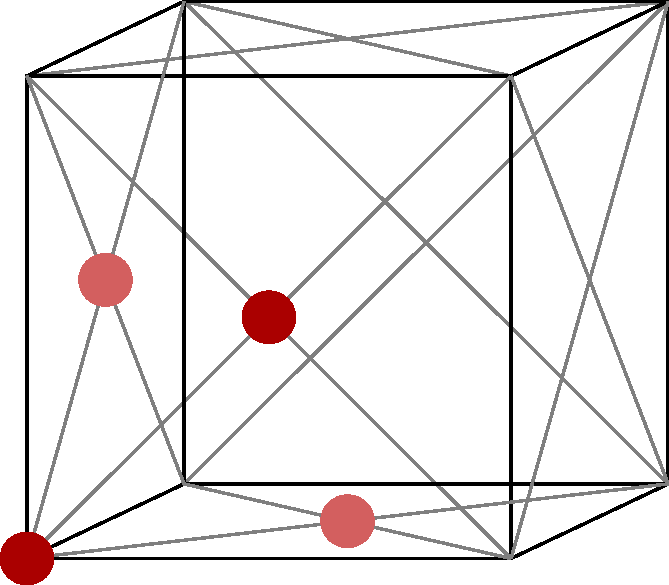
\includegraphics[scale=0.3]{images/unit_cell.pdf}
            \caption{Setup for successively building a FCC lattice}
            \label{fig:unitcell}
        \end{subfigure}
    \end{center}
\end{figure}
%\begin{figure}
    %\begin{center}
        %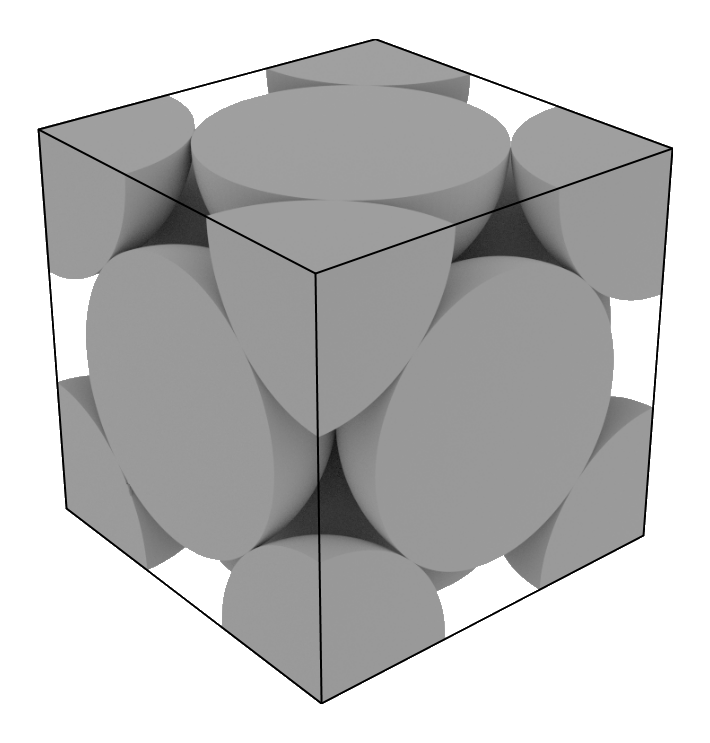
\includegraphics[scale=0.3]{images/fcc_unit.png}
        %\caption{Schematic of the number of particles contained in one FCC unit cell. The atoms on the edges are shared by 8 cells and the ones on the
            %faces by 2 cells. Image taken from
            %{https://upload.wikimedia.org/wikipedia/commons/2/27/Elementarzelle\_einer\_kubisch\_raumzentrierten\_Elementarzelle.png}}
    %\end{center}
%\end{figure}
% do i need to credit the uni buffalo course? 
% http://www.physics.buffalo.edu/phy411-506/
There are several ways to achieve this initial configuration and the one used in this thesis \cite{buffalo} was to create a kind of unit cell 
consisting of four atoms, as shown in Fig. \ref{fig:unitcell}, which can be described by a set of points
\begin{eqnarray*}
    p_1 &=& \{0,0,0\}\\
    p_2 &=& \{0.5*a,0.5*a,0\}\\
    p_3 &=& \{0.5*a,0,0.5*a\}\\
    p_4 &=& \{0,0.5*a,0.5*a\}
\end{eqnarray*}
From the particle number $N$ and the number of FCC unit cells per edge $M$ the \textit{lattice constant} $a$ can be calculated
\begin{equation}
    a = \frac{L}{M}
\end{equation}
where $L$ is the side length of the cube that is the whole system and it is calculated via the density of the system
\begin{equation}
    L = \sqrt[3]{\frac{N}{\rho}}
\end{equation}
With the lattice constant and the 4 points of the FCC cell, all the particles can be put into place.

\subsection{The Velocity-Verlet Algorithm}
\label{section:verlet}
When we look at the system from a microscopic standpoint, we see that it follows some kind of path in the phase space as time progresses. Every
point in this space corresponds to a set of positions and momenta and the connection between two points corresponds to the evolution of the system
from one state to another. As mentioned above, this evolution (the dynamics of the system) is a crucial element to molecular dynamics. Since the
equations of motion cannot be solved analytically in general, we need to approximate the solution.\\
The method used here is called finite difference approach. The trajectory of the system in the phase space is cut into finite pieces of length $\Delta
t$ and the equations of motion are solved for every segment separately (see Fig. \ref{fig:finitedifference}).\\
\begin{figure}
    \begin{center}
        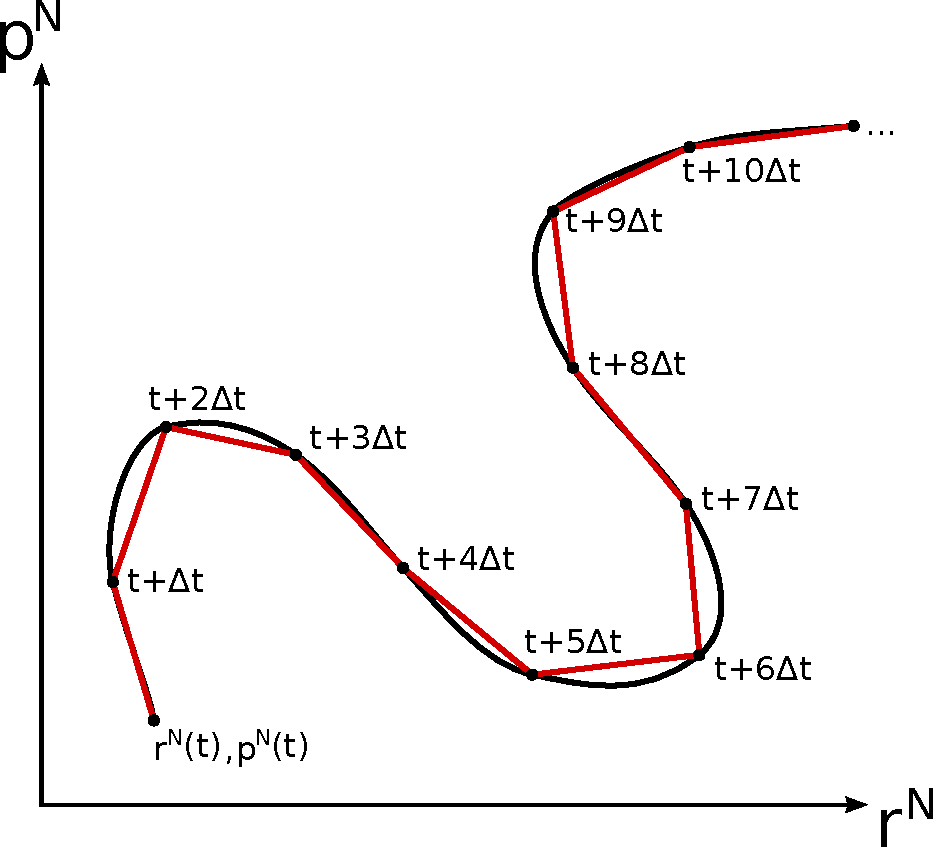
\includegraphics[scale=0.5]{images/finite_approach.pdf}
        \caption{Simplified graphical schematic of the finite difference approach. The evolution of the system from a point $(r^N(t),p^N(t))$ in the
            phase space is approximated by slicing it up into pieces of length $\Delta t$. On every stop after the starting point ($t+\Delta t$, 
            $t+2\Delta t$, $t+3\Delta t$,$\ldots$) the equations of motion can be solved numerically.}
        \label{fig:finitedifference} 
    \end{center}
\end{figure}
There are several ways to solve this kind of problem, but since we are interested in implementing it into a computer program the ideal solution
should have some basic properties \cite{Allen1989}:
\begin{itemize}
    \item It should be fast and require little memory
    \item It should permit the use of a large time step $\Delta t$
    \item It should duplicate the classical trajectory as closely as possible
    \item It should satisfy known conservation laws
    \item It should be simple and easy to program
\end{itemize}
One algorithm that has all of the above mentioned features is the one proposed by Verlet \cite{Verlet1967}. In his paper, Verlet starts by Taylor
expanding the coordinate vector $\mathbf{r}_i$ for one particle after one time step $\Delta t$:
\begin{equation}
    \label{eq:verlet}
    \mathbf{r}_i(t+\Delta t) = \mathbf{r}_i(t) + \dot{\mathbf{r}}_i \Delta t + \frac12 \ddot{\mathbf{r}}_i \Delta t^2 + \frac1{3!} \dddot{\mathbf{r}}_i \Delta t^3 +
    \mathcal{O}(\Delta t^4)
\end{equation}
Since the first derivative of the coordinate is the velocity, $\dot{\mathbf{r}}_i(t) = \mathbf{v}_i(t)$, and the second derivative of the coordinate 
is the acceleration, $\ddot{\mathbf{r}}_i(t) = \mathbf{a}_i(t)$, using Newton's law $\mathbf{F}_i(t) = m_i \mathbf{a}_i(t)$ equation \eqref{eq:verlet} 
can be written as:
\begin{equation}
    \label{eq:verletnew}
    \mathbf{r}_i(t+\Delta t) = \mathbf{r}_i(t) + {\mathbf{v}}_i(t) \Delta t + \frac1{2m} {\mathbf{F}}_i(t) \Delta t^2 + \frac1{3!} \dddot{\mathbf{r}}_i(t)
    \Delta t^3+\mathcal{O}(\Delta t^4)
\end{equation}
The same calculation can be carried out for one time step before $t$:
\begin{equation}
    \label{eq:verletnewminus}
    \mathbf{r}_i(t-\Delta t) = \mathbf{r}_i(t) - {\mathbf{v}}_i(t) \Delta t + \frac1{2m} {\mathbf{F}}_i(t) \Delta t^2 - \frac1{3!} \dddot{\mathbf{r}}_i(t) \Delta t^3+
    \mathcal{O}(\Delta t^4)
\end{equation}
The sum of those two equations yields
\begin{equation}
    \mathbf{r}_i(t+\Delta t) + \mathbf{r}_i(t-\Delta t) = 2\mathbf{r}_i(t) + \frac1{2} {\mathbf{F}}_i(t) \Delta t^2 + \mathcal{O}(\Delta t^4)
\end{equation}
and from this we get the final form for the new coordinates:
\begin{equation}
    \label{eq:verletfinal}
    \mathbf{r}_i(t+\Delta t) = 2\mathbf{r}_i(t)+ \mathbf{r}_i(t-\Delta t)+ \frac1{2} {\mathbf{F}}_i(t) \Delta t^2
\end{equation}
This means that the new coordinates can be calculated using the current coordinates, the current forces and the coordinates from the past time step.\\
From equation \eqref{eq:verletfinal} one thing becomes clear: the velocities are not necessary to calculate the new positions and they are not
computed in the process, but for the calculation of i.e. the kinetic energy the velocities are needed. Thus, the velocities have to be calculated with
a combination of the Taylor expansions of the coordinate vectors at $t+\Delta t$ and $t-\Delta t$:
\begin{equation}
    \mathbf{r}_i(t+\Delta t) - \mathbf{r}_i(t-\Delta t) = 2\mathbf{v}_i(t)\Delta t + \mathcal{O}(\Delta t^3)
\end{equation}
which can be rewritten as
\begin{equation}
    \label{eq:velocities}
    \mathbf{v}_i(t) = \frac{\mathbf{r}_i(t+\Delta t) - \mathbf{r}_i(t-\Delta t)}{2\Delta t} + \mathcal{O}(\Delta t^2)
\end{equation}
This approach has the advantage that it is fast, requires little memory and is reliable in the sense that there is no energy drift occuring during the
simulation, which means that the energy is conserved. When we compare this to the list of desired properties this seems like a good algorithm.\\
This algorithm however has two significant disatvantages. The first one is the calculation of the velocities. As can be seen in equation
\eqref{eq:velocities}, the accuracy of the calculation is only $\mathcal{O}(\Delta t^2)$ while the positions can be calculated with an error of order
$\Delta t^4$. The other big disatvantage is the first step of the algorithm. Since the calculation of the new positions requires the current positions
and the ones from one time step before, which technically do not exist.\\
The solutions to this problem is to include the stepwise calculation of the velocities \cite{swope1982}. For this we start again with the Taylor
expansion of the coordinates mathbftor \eqref{eq:verletnew} and instead of Taylor expanding $\mathbf{r}_i(t-\Delta t)$, we write it as 
\begin{equation}
    \mathbf{r}_i(t) = \mathbf{r}_i(t+\Delta t) - \mathbf{v}_i(t+\Delta t) \Delta t + \frac1{2m} \mathbf{F}_i(t+\Delta t) \Delta t^2
\end{equation}
Using \eqref{eq:verletnew} in the abvove equation we get
\begin{equation}
    \begin{aligned}
        \mathbf{r}_i(t) &= \mathbf{r}_i(t) + \mathbf{v}_i(t) \Delta t + \frac1{2m}\mathbf{F}_i(t)\Delta t^2 \\
                     &- \mathbf{v}_i(t+\Delta t) \Delta t + \frac1{2m} \mathbf{F}_i(t+\Delta t) \Delta t^2
    \end{aligned}
\end{equation}
and thus
\begin{equation}
    \label{eq:vvelocities}
    \mathbf{v}_i(t+\Delta t) = \mathbf{v}_i(t) + \frac1{2m} \left(\mathbf{F}_i(t) + \mathbf{F}_i(t+\Delta t)\right) \Delta t
\end{equation}
With the addition of this equation this algorithm is called the Velocity-Verlet algorithm, which is summarized in the following two equations:
\begin{equation}
    \label{eq:velocityverlet}
    \begin{aligned}
        \mathbf{r}_i(t+\Delta t) = \mathbf{r}_i(t) + {\mathbf{v}}_i(t) \Delta t + \frac1{2m} {\mathbf{F}}_i(t) \Delta t^2\\
        \mathbf{v}_i(t+\Delta t) = \mathbf{v}_i(t) + \frac1{2m} \Big[\mathbf{F}_i(t) + \mathbf{F}_i(t+\Delta t)\Big] \Delta t
    \end{aligned}
\end{equation}
This algorithm is self starting, uses a small amount of memory, conserves the energy (not exactly) 
and gives a very good approximation to the originial trajectory
in the phase space. To program this algorithm the following steps are needed: 
\begin{enumerate}
    \item Calculate all the forces between the particles (for the first step only)
    \item Calculate the new positions with current velocity and forces
    \item Calculate first half of the new velocities with current forces
    \item Calculate all the forces for the new position
    \item Use new forces to calculate second half of new velocities
\end{enumerate}
The first point only has to be carried out for the first step, because the forces have not been calculated at this point. As the forces are calculated
for the new positions in step 4, they can be used for the next time step. For the first time step the velocities have to be chosen randomly and are 
calculated with this algorithm from that point forward.

\subsection{The Laser Beam - Energy Influx}
The nano particle is trapped in the laser beam. While the motion of the center of mass is localized, the
individual atoms that make up the glass sphere absorb the energy from the laser which increases their velocity.\\
To simulate this kind of behaviour, thermostat algorithms \cite{Huenenberger2005} such as the Nos\'e-Hoover \cite{Nose1984,Hoover1985} or the Andersen
\cite{Andersen1980} algorithms are often used in simulation to change the temperature of the system in a controllable way.\\
The problem with these kind of algorithms is, that a target temperature has to be fixed which will be reached at some point. In order to simulate the
influx of energy from the laser it would be better to have an algorithm that supplies the system with a certain amount of energy continuously.
Fortunately, such an algorithm exists.\\
The algorithm is called Heat Exchange Algorithm (HEX) \cite{Hafskjold1993}. Its intended purpose is the use in non-equilibrium molecular dynamics
(NEMD) to study transport phenomena and determine transport coefficients. The algorithm works by introducing two regions in the system, one serving as
a heat source and the other as a heat sink. A specific amount of heat is then exchanged between those two reservoirs. As it turns out however, this
algorithm introduces an energy shift for longer simulation times. This led Wirnsberger et al. \cite{Wirnsberger2015} to revisit the algorithm and 
identify the cause of this energy drift, to create a more suitable algorithm, which they called eHEX.\\
As in the HEX algorithm, regions are introduced to the system which act either as heat sinks or heat sources. These are labelled with $\Gamma_k$,
where $k > 0$, and have corresponding amount of exchanged heat $\Delta Q_{\Gamma_k}$. If $\Delta Q_{\Gamma_k}$ is negative, heat is subtracted from
the system and vice versa. Regions that neither act as heat source or heat sink are labelled with $\Gamma_0$, which are also called
Hamiltonian regions (see Fig. \ref{fig:ehex}). 
\begin{figure}
    \begin{center}
        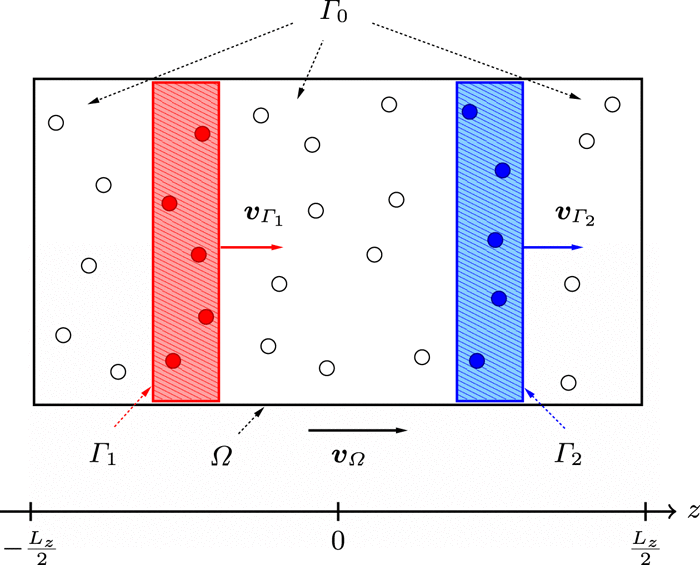
\includegraphics[scale=0.3]{images/ehex_system.png}
        \caption{Setup for the use of the HEX and eHEX algorithms. The simulationbox $\Omega$, which is moving with a velocity of $v_\Omega$,
        contains a heat source (red), $\Gamma_1$, which is moving with velocity $v_{\Gamma_1}$ and a heat sink (blue), $\Gamma_2$, which is moving 
        with velocity $v_{\Gamma_2}$. The regions that are neither heat sources or heat sinks are denoted by $\Gamma_0$.}
        \label{fig:ehex} 
    \end{center}
\end{figure}
The centers of mass of the particles in simulation box, denoted by $\Omega$, and the regions $\Gamma_k$ 
are assumed to be moving with velocities $v_\Omega$ and $v_{\Gamma_k}$ respectively.\\
The change of the energy in a region $\Gamma_k$ is achieved by rescaling the velocities by a factor $\xi_k$ and shifted by the velocity of the
corresponding region:
\begin{equation}
    \mathbf{v}_i \rightarrow \mathbf{\bar{v}}_i = \xi_k \mathbf{v}_i + (1-\xi_k)\mathbf{v}_{\Gamma_k}
\end{equation}
The bar over a quantity denotes the value after the exchange of heat.\\
The factor $\xi_k$ is given by
\begin{equation}
    \xi_k = \sqrt{1+\frac{\Delta Q_{\Gamma_k}}{\mathcal{K}_{\Gamma_k}}}
\end{equation}
where $\Delta Q_{\Gamma_k}$ is the exchanged heat in the region $\Gamma_k$ and $\mathcal{K}_{\Gamma_k}$ is the non-translational kinetic energy of the
region $\Gamma_k$ and is given by
\begin{equation}
    \label{eq:kineticK}
    \mathcal{K}_{\Gamma_k} = \sum_{i \in \gamma_k} \frac{m_i v_i^2}{2} - \frac{m_{\Gamma_k}v_{\Gamma_k}^2}{2}
\end{equation}
The sum is taken over all indices in $\gamma_k$ which is the set of indices of particles in the region $\Gamma_k$.\\
For the final version of the eHEX algorithm there are three more quantities needed. The first one is the heat flux per time step, denoted by 
$\mathcal{F}_\GammaK$:
\begin{equation}
    \mathcal{F}_\GammaK = \frac{\Delta Q_\GammaK}{\Delta t}
\end{equation}
The second one is the thermostatting force $\boldsymbol{\eta}_i$, which is defined as
\begin{equation}
    \boldsymbol{\eta}_i = 
    \begin{cases}
        m_i \ \dfrac{{\mathcal{F}_{\Gamma_{k(\mathbf{r}_i)}}}}{{2\mathcal{K}_{\Gamma_{k(\mathbf{r}_i)}}}} \
        \left(\mathbf{v}_i - \mathbf{v}_{\Gamma_{k(\mathbf{r}_i)}}\right)
        & \quad \text{if } k(\mathbf{r}_i) > 0 \\
        0 & \quad \text{otherwise}
    \end{cases}
    %\begin{cases}
        %m_i \ \frac{\displaystyle{\mathcal{F}_{\Gamma_{k(\mathbf{r}_i)}}}}{\displaystyle{2\mathcal{K}_{\Gamma_{k(\mathbf{r}_i)}}}} \
        %\left(\mathbf{v}_i - \mathbf{v}_{\Gamma_{k(\mathbf{r}_i)}}\right)
        %& \quad \text{if } k(\mathbf{r}_i) > 0 \\
        %0 & \quad \text{otherwise}
    %\end{cases}
\end{equation}
where $k(\mathbf{r}_i)$ is the index of the region in which particle $i$ located, i.e. $k(\mathbf{r}_i) = 0$ means that the particle is in a Hamiltonian
region and $k(\mathbf{r}_i) > 0$ denotes the heat sinks and sources.\\
The last quantity is the one that corrects the long term energy drift of the HEX algorithm, denoted by $\mathcal{E}{r}_{i,\alpha}$.
The analysis and derivation of this term is given in \cite{Wirnsberger2015}.
\begin{equation}
    \label{eq:bigeps}
    \begin{aligned}
        \mathcal{E}{r}_{i,\alpha} &= \dfrac{\eta_{i,\alpha}}{m_i\mathcal{K}_{\Gamma_{k(\mathbf{r}_i)}}} \left[
        \frac{\mathcal{F}_{\Gamma_{k(\mathbf{r}_i)}}}{48} + \frac{1}{6} \sum_{j\in\gamma_{k(\mathbf{r}_i)}} \mathbf{f}_j \cdot \left(\mathbf{v}_j - 
            \mathbf{v}_{\Gamma_{k(\mathbf{r}_i)}}\right)\right] \\
            &- \frac{\mathcal{F}_{\Gamma_{k(\mathbf{r}_i)}}}{12\mathcal{K}_{\Gamma_{k(\mathbf{r}_i)}}} \left[
            \frac{f_{i,\alpha}}{m_i} - \frac{1}{m_{\Gamma_{k(\mathbf{r}_i)}}} \sum_{j\in\gamma_{k(\mathbf{r}_i)}}f_{j,\alpha}\right]
    \end{aligned}
\end{equation}
The $\mathbf{f}$ in the above equation denotes the force corresponding to the chosen intermolecular potential $U(\mathbf{r})$, 
\begin{equation}
    \mathbf{f} = -\nabla_{\mathbf{r}_i} U(\mathbf{r}_i)
\end{equation}
With all the necessary quantities established, the updating sequence of the eHEX algorithm can be written down:
\begin{subequations}
\begin{eqnarray}
    \bar{\mathbf{v}}^n_i &=& \xi^n_{k(\mathbf{r}_i)} \mathbf{v}^n_i + \left(1-\xi^n_{k(\mathbf{r}_i)}\right) \mathbf{v}^n_{\Gamma_{k(\mathbf{r}_i)}} \\
    \bar{\mathbf{v}}^{n+\frac12}_i &=& \bar{\mathbf{v}}^n_i + \frac{\Delta t}{2m_i} \mathbf{f}^n_i\\
    \bar{\mathbf{r}}^{n+1}_i &=& \mathbf{r}^n_i + \Delta t \bar{\mathbf{v}}^{n+\frac12}_i\\
    \mathbf{f}^{n+1}_i &=& \left.-\nabla_{\mathbf{r}_i} U(\mathbf{r})\right|_{\mathbf{r} = \bar{\mathbf{r}}^{n+1}}\\
    \bar{\mathbf{v}}^{n+1}_i &=& \bar{\mathbf{v}}^{n+\frac12}_i + \frac{\Delta t}{2m_i} \mathbf{f}^{n+1}_i\\
    \mathbf{v}^{n+1}_i &=& \bar{\xi}^{n+1}_{k(\bar{\mathbf{r}}_i)} \bar{\mathbf{v}}^{n+1}_i + \left(1-\bar{\xi}^{n+1}_{k(\bar{\mathbf{r}}_i)}\right)
    \bar{\mathbf{v}}^{n+1}_{\Gamma_{k(\bar{\mathbf{r}}_i)}} \\
    \mathbf{r}^{n+1}_i &=& \bar{\mathbf{r}}^{n+1} - \Delta t^3 \mathcal{E}\bar{\mathbf{r}}^{n+1}_i
\end{eqnarray}
\end{subequations}
This algorithm can be adapted for the problem of the levitating nano sphere in the laser beam by adjusting the setup and some of the parameters.\\
Firstly, the setup of the heat sinks and sources has to be changed. Since there is only energy pumped into the system from the outside, the region
acting as a heat sink vanishes and the region acting as a heat source spans over the whole simulation box. This means that, using the 
notation of Fig. \ref{fig:ehex}, $\Omega = \Gamma_1$. Furthermore, neither center of mass of the particles the simulation box nor 
the heat source are moving, i.e. 
$\mathbf{v}_\Omega = \mathbf{v}_{\Gamma_1} = 0$. This affects the non-translational kinetic energy term $\mathcal{K}_{\Gamma_1}$, the thermostatting
force $\boldsymbol{\eta}$ and the correction term $\mathcal{E}\mathbf{r}$. Since there is only one region acting as a heat source, the terms $\Delta Q$,
$\mathcal{K}$ and $\mathcal{F}$ don't need an index. The summation index in \eqref{eq:kineticK} and \eqref{eq:bigeps} can be changed to the number of
particles in the system, $N$, since all the particles are within the heat exchanging region. The masses are set to 1, i.e. $m_i = 1$ with the chosen
reduced units and with this the total mass of the region (in the term $1/m_{\Gamma_{k(\mathbf{r}_i)}}$ in \eqref{eq:bigeps}) is equal to the number of
particles in the system. With these changes, the quantities can be written down as:
\begin{eqnarray}
    \mathcal{K} &=& \sum_{N} \frac{v_i^2}{2}\\
    \xi &=& \sqrt{1+\frac{\Delta Q}{\mathcal{K}}}\\
    \mathcal{F} &=& \frac{\Delta Q}{\Delta t}\\
    \boldsymbol{\eta}_i &=& 
    \dfrac{\mathcal{F}}{{2\mathcal{K}}} \
        \mathbf{v}_i\\
        \mathcal{E}{r}_{i,\alpha} &=& \dfrac{\eta_{i,\alpha}}{\mathcal{K}} \left[
        \frac{\mathcal{F}}{48} + \frac{1}{6} \sum_{N} \mathbf{f}_j \cdot \mathbf{v}_j
            \right] \nonumber \\
            &-& \frac{\mathcal{F}}{12\mathcal{K}} \left[
            {f_{i,\alpha}} - \frac{1}{N} \sum_{N}f_{j,\alpha}\right]
\end{eqnarray}
This means that the laser is modeled to be pumping energy into the system, which increases the velocities of the particles in the
system over time, while the center of mass motion is not affected by this.\\


\subsection{The Laser Beam - Trapping}
As mentioned above, the glass particle is trapped in the laser beam and the position of the particle is localized. This behaviour
has to be modeled as well.\\
The approximation of the original paper \cite{Gieseler2014}, where the movements in the three spatial directions are decoupled will be
used in the model as well. As to the model of the trapping force itself, the most straightforward approach is to use a harmonic oscillator potential.
The force and the corresponding potential can be written as
\begin{eqnarray}
    \mathbf{F} &=& -k \Big[\mathbf{x}-\mathbf{x}_0\Big]\\
    U &=& \frac12 k \Big[\mathbf{x}-\mathbf{x}_0\Big]^2
\end{eqnarray}
where $\mathbf{x}_0$ is the position of minimal potential energy. 
Since the trap is acting on the whole system, the force is acting on the center of mass. 
To calculate the center of mass positions and velocities, the positions and velocities of all particles have to be summed up and 
divided by the particle number:
\begin{equation}
    \mathbf{r}_\text{COM} = \frac1N\sum_{i=1}^N \mathbf{r}_i
\end{equation}


\subsection{Surrounding Gas - Thermostat}
Without any equilibrating mechanism the setup described by now would lead to the system heating up indefinetly, which is not desirable. Furthermore,
the goal is to recreate the experiment as close as possible. Since the nano particle is trapped in a laser beam within a vacuum chamber, the
surrounding gas has to be modeled as well. In the next step we will introduce the surrounding gas of the gas chamber that will absorb some of the 
energy in the system, leading to the final state.\\
Generally, pressure is introduced to the system by surrounding the object of interest (in this case the glass nano sphere) with a thermostatting
pressure medium.
There are two main requirements for the choice of such a pressure medium: the exerted pressure must be hydrostatic and the computation of the
interaction between the pressure medium and the object of interest must not take up a lot of resources.\\
The model used in this thesis was developed by Gr\"unwald and Dellago \cite{Gruenwald2006} and uses an ideal gas of non-interacting particles as
thermostatting pressure medium. The particles of this pressure medium flow into the simulation from an outside volume, whose geometry is based on the form of the
object of interest (this will be referred to as the minimal volume of cells) and leave the simulation box if their position reaches the boundary of
this minimal volume of cells. This behaviour is very close to the real experiment which makes this thermostat an ideal candidate for the simulation of
the experiment. 
%This barostat also acts as a thermostat and thus is suitable for the 
%application in this thesis.\\
The gas particles interact with the object via a soft-sphere potential of the form
\begin{equation}
    \label{eq:softsphere}
    U(r) = \varepsilon \left(\frac{\sigma}{r}\right)^{12}
\end{equation}
where $\varepsilon$ is the interaction strength and $\sigma$ is the interaction range and $r$ is the distance between the gas particle and the
interacting particle. The gas particles do not interact with one another in this model.\\
In order to increase the efficiency of the computing process, $\sigma$ should be chosen carefully. For larger $\sigma$, the number of interaction
partners increases, which increases the number of force calculations which are a very time consuming part. For smaller $\sigma$ the possibility for
gas particles reaching the inside of the nano particle increases, which is not desirable. So $\sigma$ should be chosen small enough to keep the force
calculations at a minimum and large enough for the particle to stay on the outside of the crystal. In the computer simulations performed for this
thesis, the interaction length is chosen to be $\sigma = 1$ with a cut-off radius of $r_c = 2.5$.\\ 
The algorithm can be performed by following these steps:
\begin{enumerate}
    \item Randomly draw the number of particles that are created on a single side of the minimal volume of cells, $N_\text{fac}$, from the
        distribution 
        \begin{equation}
            %\langle N_\text{fac}\rangle = \Delta t L^2 P \left(\frac{1}{2\pi m k_B T}\right)^\frac12
            \langle N_\text{fac}\rangle = \Delta t L^2 P \sqrt{\frac{1}{2\pi m k_B T}}
        \end{equation}
        where $\Delta t$ is the time step of the simulation, $L$ is the side length of the cell in which the particle is created, $P$ is the desired
        pressure, $m$ is the mass of the gas particle, $k_B$ is the Boltzmann constant (which will be set to 1 in reduced units) and $T$ is the
        desired temperature. This chosen number of particles is then equally distributed over the face of the cell on which they are created. The
        velocities of the created particles are drawn from two different random number distributions. The component of the particle perpendicular to
        the surface is drawn from a Rayleigh distribution of the form 
        \begin{equation}
            p(v_i) = \frac{m}{k_B T}v_i \ e^{-\frac{mv_i^2}{2k_BT}}
        \end{equation}
        The other components of the particles' velocity are drawn from a Maxwell-Boltzmann distribution.
    \item Perform the first step of the velocity Verlet algorithm to propagate the particle positions by one time step.
    \item Check if any gas particles have left the minimal volume of cells and remove those which have.
    \item Check if the geometry of the crystal and with it the minimal volume of cells has changed. If it has, remove all gas particles in the cells
        that are no longer needed. Then insert new gas particles to the created cells with a number drawn from a Poisson distribution with mean value
        \begin{equation}
            \langle N_\text{ins}\rangle = \frac{PL^3}{k_BT}
        \end{equation}
        If the length of the cell $L$ is chosen to be equal to the cut-off radius $r_c$, this insertion should only be carried out with a probablity of
        \begin{equation}
            P_\text{ins} = e^{-\frac{U}{k_BT}}
        \end{equation}
        (where U is the interaction energy between the gas particle and the crystal) because it is possible that the inserted particle is 
        within the interaction range of the crystal. 
    \item Compute all forces.
    \item Perform the second step of the velocity Verlet and propagate the particle velocities by one time step. 
\end{enumerate}
This algorithm is formulated in a general fashion, so that a wide range of crystals and geometries can be used. 
%The setup used in this thesis is a FCC lattice, which has a nice symmetry that is not influenced by the surrounding gas. 
Although the shape of the nano particle changes over the course of the simulation, it is not necessary to change the geometry of the surrounding box.
The algorithm will therefore not be carried out using cell-lists and a minimal volume of cells that is changing over the course of the simulation, 
but rather a fixed setup of the volume surrounding the nano particle.\\ 
Since the particle itself is modeled as a cube, a straighforward approach is surrounding it by a bigger cube. The distance between the cube face and the nano
particle is chosen to be the side length of the nano particle, so the setup will properly scale for different numbers of particles. 
The schematic setup for this is depicted in Fig.\ref{fig:gascube}.
\begin{figure}[h]
    \begin{center}
        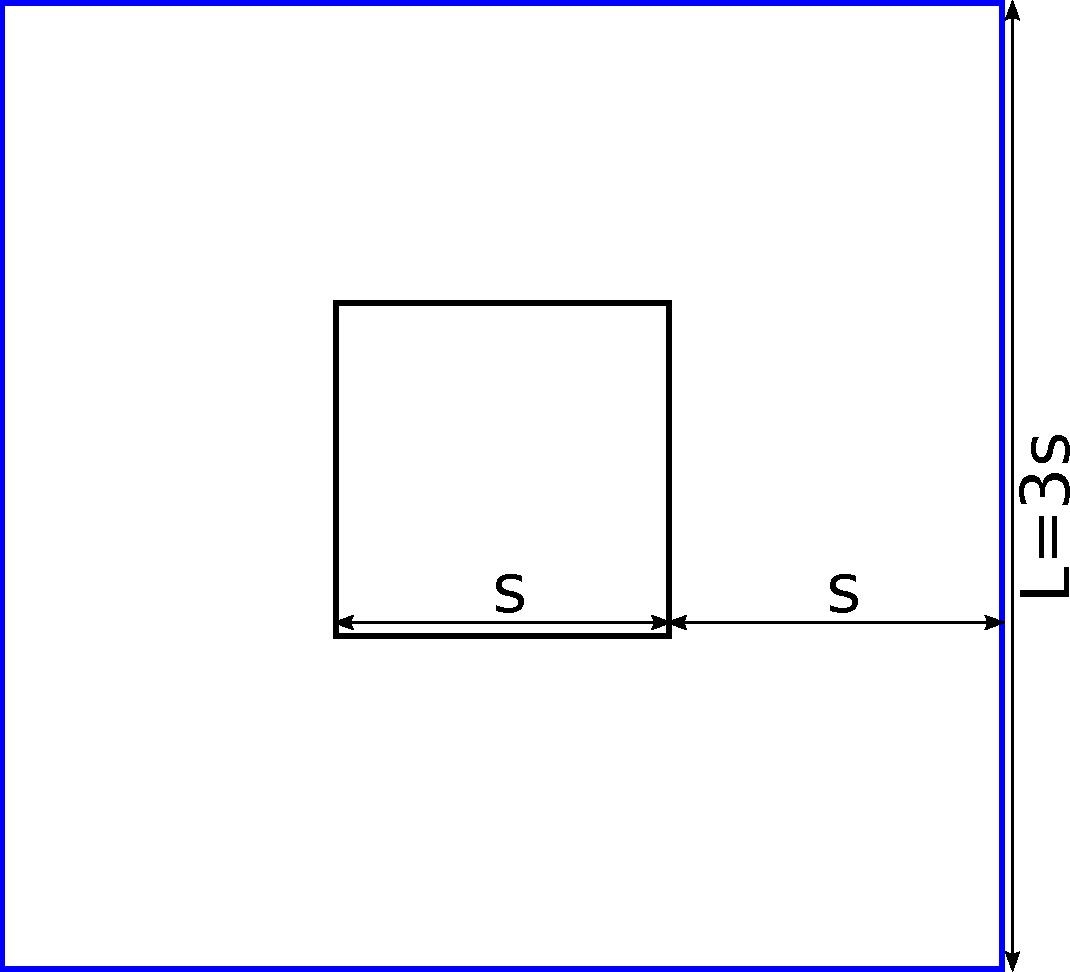
\includegraphics[scale=0.5]{images/gas_volume_ver3.pdf}
        \caption{Schematic setup for the barostat. The outer volume (blue) is one side length $s$ away from the nano particle (black) which means that
            the side length of the face of the surrounding box is $L=3s$. 
                    The gas particles are created along the blue lines of the outer volume. Since the overall geometry of the nano particle does 
                    not change, 
                    the geometry of the outer volume will be constant throughout the simulation.}
        \label{fig:gascube}
    \end{center}
\end{figure}


%This is done by adding for instance two regions to the simulation, one providing an influx of heat
%and the other acting as a heat sink. The algorithm is furthermore designed to incorporate the velocities of the center of mass of the system and the
%velocities of the regions. 


%\subsection{The Glass Nanoparticle}
%The glass particle from the experiment will be represented by a system of 864 particles, aligned regularly on a FCC (face centered cubic) lattice.
%This alignment is achieved by defining a minimum cell, containing points:
%\begin{eqnarray*}
    %p_1 &=& \{0,0,0\}\\
    %p_2 &=& \{0.5,0.5,0\}\\
    %p_3 &=& \{0.5,0,0.5\}\\
    %p_4 &=& \{0,0.5,0.5\}
%\end{eqnarray*}
%The whole system is then  created by copying this unit cell.\\
%The interaction between the atoms is modeled by the Lennard-Jones potential. It has the form
%\begin{equation}
    %U(r) = 4\varepsilon\left[\left(\frac\sigma r\right)^{12} - \left(\frac\sigma r\right)^6\right].
%\end{equation}
%To simplify the equation and computation of the potential and other quantities, like the forces or pressure, it is useful to introduce reduced units.
%In general, reduced units BLABLABLA THINK OF GOOD TEXT HEREJKA\\
%The basic units in a system with Lennard-Jones interaction are length ($\sigma$), energy ($\varepsilon$ or $\varepsilon / k_B$) and mass ($m$). Every 
%quantity can now be written in terms of this units, so they become reduced quantities, denotet by an asterisk. The most important ones are:
%\begin{eqnarray*}
    %r^* &=& r/\sigma\\
    %T^* &=& k_B/\varepsilon \ T\\
    %U^* &=& U/\varepsilon \\
    %P^* &=& P \sigma^3/\varepsilon 
%\end{eqnarray*}
%With the above introduced reduced units, the Lennard-Jones potential can be written as
%\begin{equation}
    %U(r^*) = 4\left[{r^*}^{-12} - {r^*}^{-6}\right].
%\end{equation}
%Since this is the most practical form, it will be used without the asterisk from here on.\\
%The Lennard-Jones potential is an additive pair-potential, so the total energy of the system can be calculated by summing over all pairs of atoms:
%\begin{equation}
    %U_{\text{tot}} = \sum_{i=1}^{N-1}\sum_{j=i+1}^N4\left[{r_{ij}}^{-12} - {r_{ij}}^{-6}\right]
%\end{equation}
%where $r_{ij}$ denotes the distance between atom $i$ and $j$. \\
%The Velocity-Verlet algorithm uses the forces to calculate the positions and velocities for the next timestep, we need to calculate the derivative of
%the potential energy:
%\begin{eqnarray}
    %F_{x} &=& -\frac{\partial}{\partial x} U(r) \nonumber\\
                %&=& -\frac{\partial}{\partial x} 4\left[{r}^{-12} - {r}^{-6}\right] \nonumber\\
                %&=& -4 \left[(-12){r}^{-13} - (-6){r}^{-7}\right] \frac{\partial r}{\partial x} \nonumber\\
                %&=& 48 \left[r^{-13} - 0.5 \ r^{-7}\right] \frac{x}{r} \nonumber\\
    %\label{eq:ljforce} &=& 48 \left[r^{-14} - 0.5 \ r^{-8}\right] x
%\end{eqnarray}
%This is the component of the force in x-direction -- the other components are calculated analogously.






\newpage
\section{Results}
% results with different parameters, graphs, etc.
Since the simulation consists of various parts that have to work together, we first need to check if every part itself works.\\
\subsection{The Crystal}
The first element of the simulation is the setup of the FCC lattice on which the particles are placed on. To check if this is done correctly, we can
use a visualisation and rendering software such as VMD\cite{Humphrey1996} or OVITO\cite{Stukowski2010}. The rendered image of the nano particle 
can be seen in Fig.~\ref{fig:glass}. The chosen perspective shows the structure of the FCC lattice, where 3 layers are forming 
where the atoms take the position on the gap between the atoms from the layer below.\\
\begin{figure}[h]
    \begin{center}
        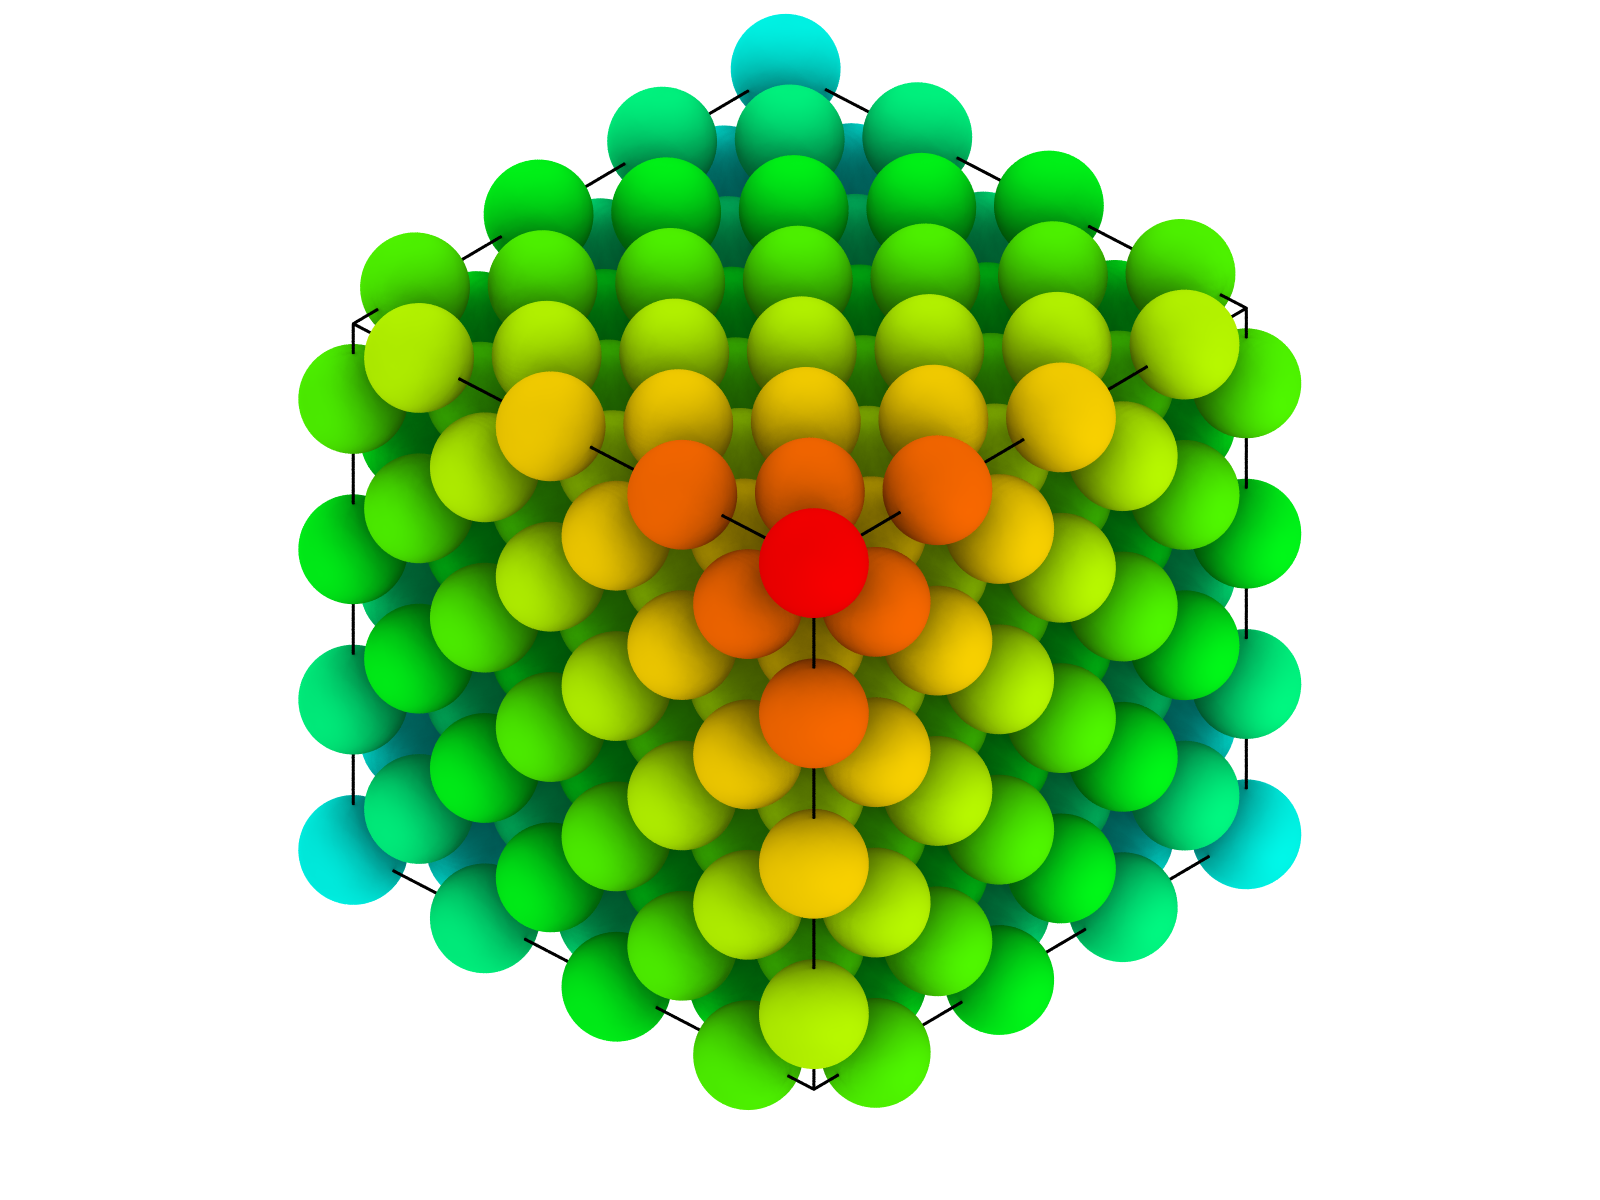
\includegraphics[scale=0.2]{images/fcc_rendering_layer_newcoloring.png}
        \caption{A rendered image of the FCC lattice. The chosen color-coding along the (1,1,1) Miller-index 
                highlights the layers for this perspective. The perspective is
                chosen to see the layering of the FCC lattice with its 3 layer structure. The black box acts as a reference point to outline the 
                geometry of the system.}
            %Rendering of the model of the nano crystal before starting the simulation. 
            %The chosen perspective shows the 3 layers of the FCC crystal with a
                    %These layers consist of atoms
                    %taking the position above the gap between two of the atoms from the layer below and match the positions of the atoms 2 layers
                %below. The black box is the outline of the particles' positions and shows the geometry of the system.}
        \label{fig:glass}
    \end{center}
\end{figure}

\subsection{Velocity Verlet}
The velocity Verlet part of the simulation is taking place in a NVE ensemble from a thermodynamic point of view. 
This means that the particle number $N$, the volume $V$ and the total energy $E$ are constant. 
The initial velocities of the particles are chosen randomly from a Maxwell-Boltzmann distribution. To ensure that the system behaves the way it is
intended to, small adjustments have to be made in the beginning of the simulation of the nano particle.\\
%In contrast to the NVT ensemble used in Monte-Carlo simulations this means, that the velocities of the particle can not
%be chosen directly. The initial velocities have to be drawn from a random number generator. This means that the velocities have to be adjusted after 
%they have been drawn.\\
The first adjustment that needs to be made is making sure that the system is staying in place and not floating away. To do this, the velocity vectors
of all the atoms in the system have to be added to get the resulting velocity vector for the whole system. 
This resulting vector is then divided by the number of particles in the system and the resulting vector is then subtracted from every
velcocity vector of every atom in the system. 
\begin{eqnarray}
    \mathbf{v}_\text{tot} &=& \sum_{i=1}^N \mathbf{v}_i\\
    \mathbf{v}_\text{cut} &=& \frac{\mathbf{v}_\text{tot}}N\\
    \mathbf{v}_i^\text{new} &=& \mathbf{v}_i - \mathbf{v}_\text{cut}
\end{eqnarray}
This adjustment only needs to be done just after randomly choosing the velocities, as there is no force present at this point that would cause the
nano particle to move.
%The next adjustment is a small one that makes a difference in the long run. When choosing random velocities, the system not only tends to have a
%resulting velocity vector that causes the whole system to float away, but also a resulting angular momentum that causes the system to rotate.
%The angular momentum can be defined via the moment of inertia $\mathbf{I}$
%\begin{eqnarray}
    %\label{eq:angularmomentum}\mathbf{L} &=& \mathbf{I}\boldsymbol{\omega}\\
    %\boldsymbol{\omega} &=& \frac{\mathbf{r} \times \mathbf{v}}{r^2}
%\end{eqnarray}
%where $\boldsymbol{\omega}$ is the angular velocity of the system. Another way to define the angular momentum is given by
%\begin{equation}
    %\label{eq:angularmomentum2}
    %\mathbf{L} = \mathbf{r} \times \mathbf{p}
%\end{equation}
%where $\mathbf{p}$ is the momentum of the particle, which in this case is equal to its velocity since the mass is set to 1.The moment of inertia 
%$\mathbf{I}$ for a filled cube is given by 
%\begin{equation}
    %\mathbf{I} = 
    %\begin{pmatrix}
        %\frac{mL^2}{6} & 0 & 0\\
        %0 & \frac{mL^2}{6} & 0\\
        %0 & 0 & \frac{mL^2}{6} 
    %\end{pmatrix}
%\end{equation}
%where $m$ will be later set to 1 and $L$ is the side length of the cube. To use this equations to suppress the rotation of the cube, we need to use
%equation~\eqref{eq:angularmomentum} and rewrite it as
%\begin{equation}
    %\label{eq:omega}
    %\boldsymbol{\omega} = \mathbf{I}^{-1}\mathbf{L}
%\end{equation}
%where $\mathbf{I}^{-1}$ is the inverse matrix of $\mathbf{I}$. The calculation of the inverse matrix is fairly straightforward, as it only contains
%values in the diagonal, which means that the inverse matrix can be calculated by simply inverting these values. The angular momentum for every
%particle $\mathbf{L}_i$ in the above equation be calculated using eq.~\eqref{eq:angularmomentum2}, where the position is taken to be the distance
%between the particle and the center of mass
%\begin{equation}
    %\Delta\mathbf{r}_i = \mathbf{r}_\text{COM} - \mathbf{r}_i
%\end{equation}
%The values of the angular momentum for each paricle are added up and multiplied by the inverse of the moment of inertia, as described in
%eq.~\eqref{eq:omega}. The final step is updating the velocities of the particles:
%\begin{equation}
    %\mathbf{v}_i^\text{new} = \mathbf{v}_i - \left(\boldsymbol{\omega} \times \Delta\mathbf{r}_i\right)
%\end{equation}
%\\The velocities of the particle can roughly be chosen by adjusting the range of numbers the random number generator can choose from. However, the
%resulting velocities (and therefore the temperature of the system) are generally not precisely how they should be. 
\\As mentioned above, the velocities are chosen from a Maxwell-Boltzmann distribution, which means choosing each component from a Gaussian
distribution. However, the positions on the FCC lattice are not very natural and so the atoms equilibrate to a different temperature than desired.
If the system should have a
specific starting temperature $T$, the velocities need to be scaled accordingly. This rescaling is done by summing the square of the velocities
(this equals calculating the kinetic energy since the masses are set to 1) and rescale them by a factor $\lambda$:
\begin{eqnarray}
\label{eq:rescale1}   E &=& \sum_{i=1}^N \frac{\mathbf{v}_i^2}{2} \\
 \label{eq:rescale2}   \lambda &=& \sqrt{\frac{3(N-1)T}{2E}} \\
 \label{eq:rescale3}   \mathbf{v}_i^\text{new} &=& \lambda \mathbf{v}_i  
\end{eqnarray}
This process has to be done a couple of times, until the system equilibrates to the desired temperature. 
%The problem with this procedure is the fact
%that it is not compatible with the requirement of constant energy of the system. 
If we look at the energy values in Fig.~\ref{fig:energystart} we can see the
irregularities (jumps) before the system equilibrates to a constant value. This equilibration process divides the simulation in two phases: the equilibration
phase and the measurement phase. In the equilibration phase, the system has time to reach a configuration that is (as the name suggests) in an 
equilibrated state. During this phase, there are usually no measurements (such as energy) performed, since the values from this phase are distorting
the mean value of the simulation. That is why the configurations from the equilibration phase are discarded and the measurement phase takes place, 
where the values do get calculated and are used to determine the mean values.  
\begin{figure}[h]
    \begin{center}
        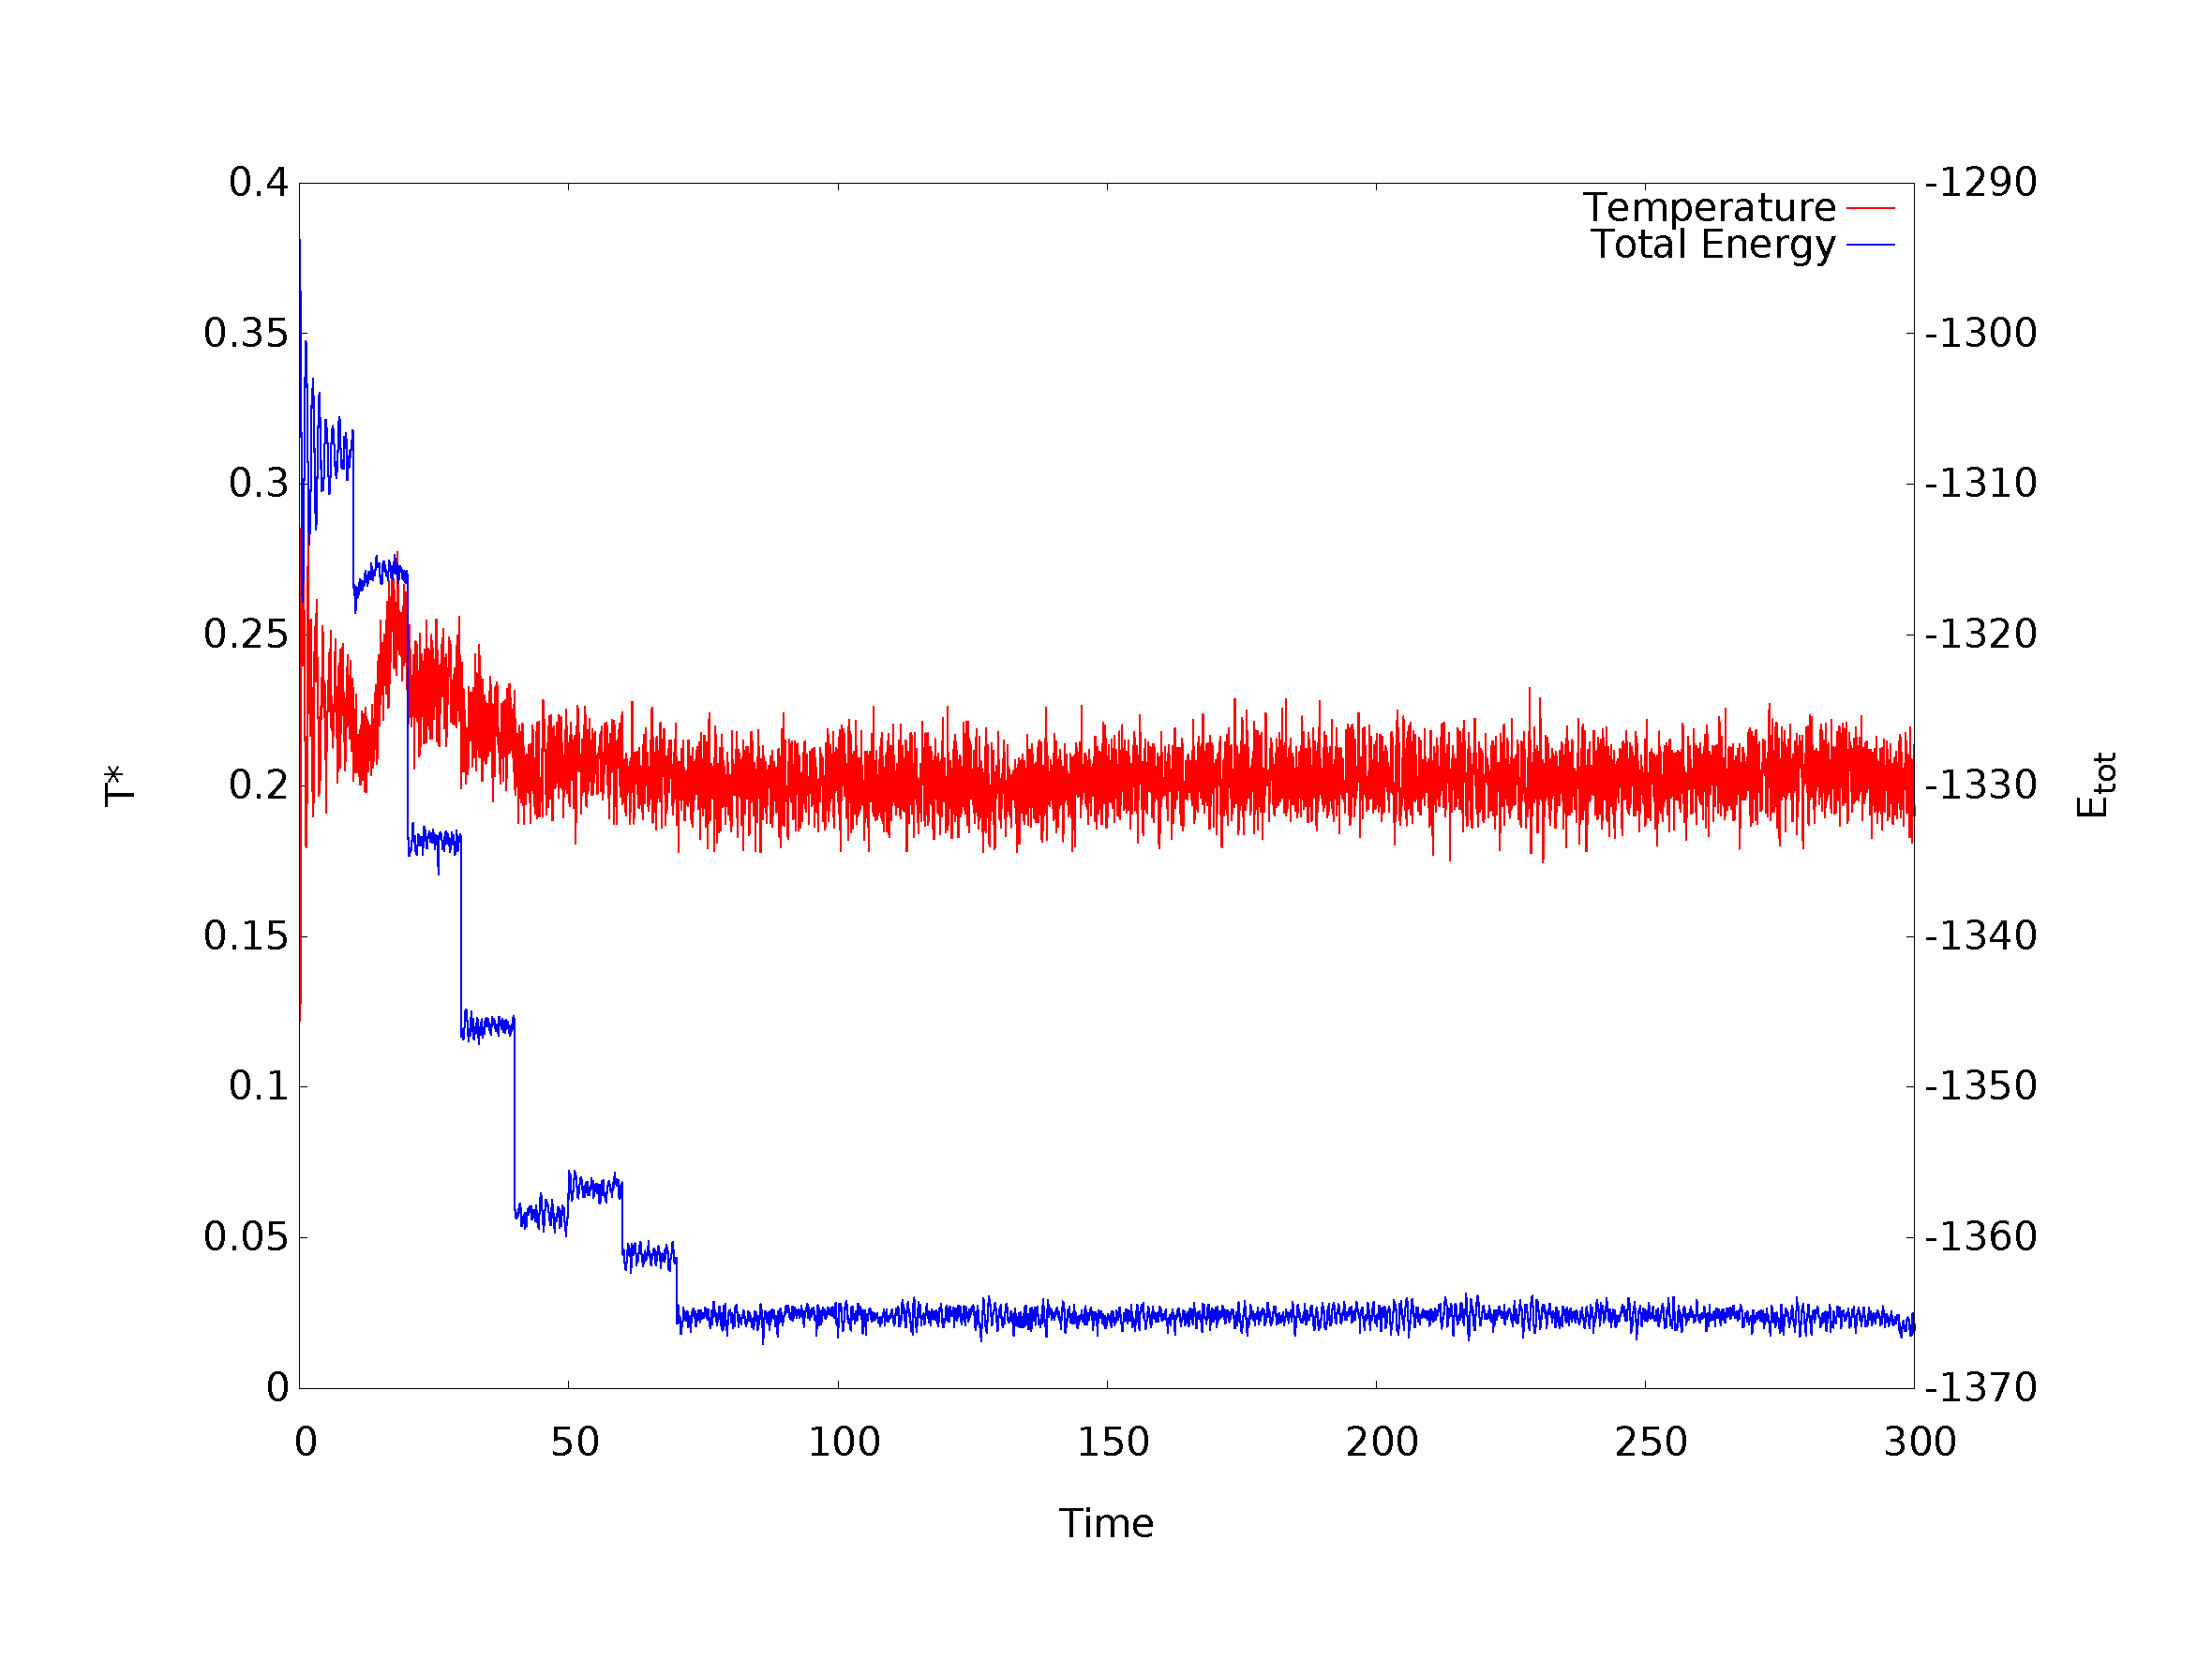
\includegraphics[scale=0.3]{images/verlet_output_te.pdf}
        \caption{Temperature and energy in the equilibration phase of the velocity Verlet algorithm. The velocity rescaling (see eq. 
        \eqref{eq:rescale1}-\eqref{eq:rescale3}) is taking place every 1000th step until the 9000th, which can be seen in the energy curve whre the
    jumps are happening. The desired temperature in this case is $T^* = 0.2$, which is reached after about 7000 steps.}
        \label{fig:energystart}
    \end{center}
\end{figure}

\subsection{eHEX}
The next checkpoint is the eHEX algorithm. Since it contains several steps and variables that have to be calculated, this algorithm is very prone
to errors. Perhaps the most crucial of those variables in the algorithm is the amount of heat injected into the system, $\Delta Q$. 
The effect of the value of this variable on the system has therefore to be checked to make sure the system is not overheating.\\
The investigation of the effects on the system can be done in two ways: comparing the temperature and the energy of the system during the 
application of the algorithm (similar to the way it's been done with the velocity Verlet) and comparing the effect of different values of $\Delta Q$.\\
%Like mentioned above, there is an equilibration phase, which takes place before the recording of the values for this comparison. The graph starts 
%with a velocity Verlet phase after which the eHEX algorithm starts, to emphasize the effect of the change in temperature and energy.\\
Since the eHEX algorithm injects heat into the system, one would expect the energy and the temperature to rise during the application of the
algorithm. In Fig.~\ref{fig:ehex_te} we can see that exactly this is happening. The graph shows a velocity Verlet phase (that follows an equilibration
phase which is not recorded) of constant temperature and energy and an eHEX phase, where the temperature and the enrgy are constantly rising. 
\begin{figure}[h]
    \begin{center}
        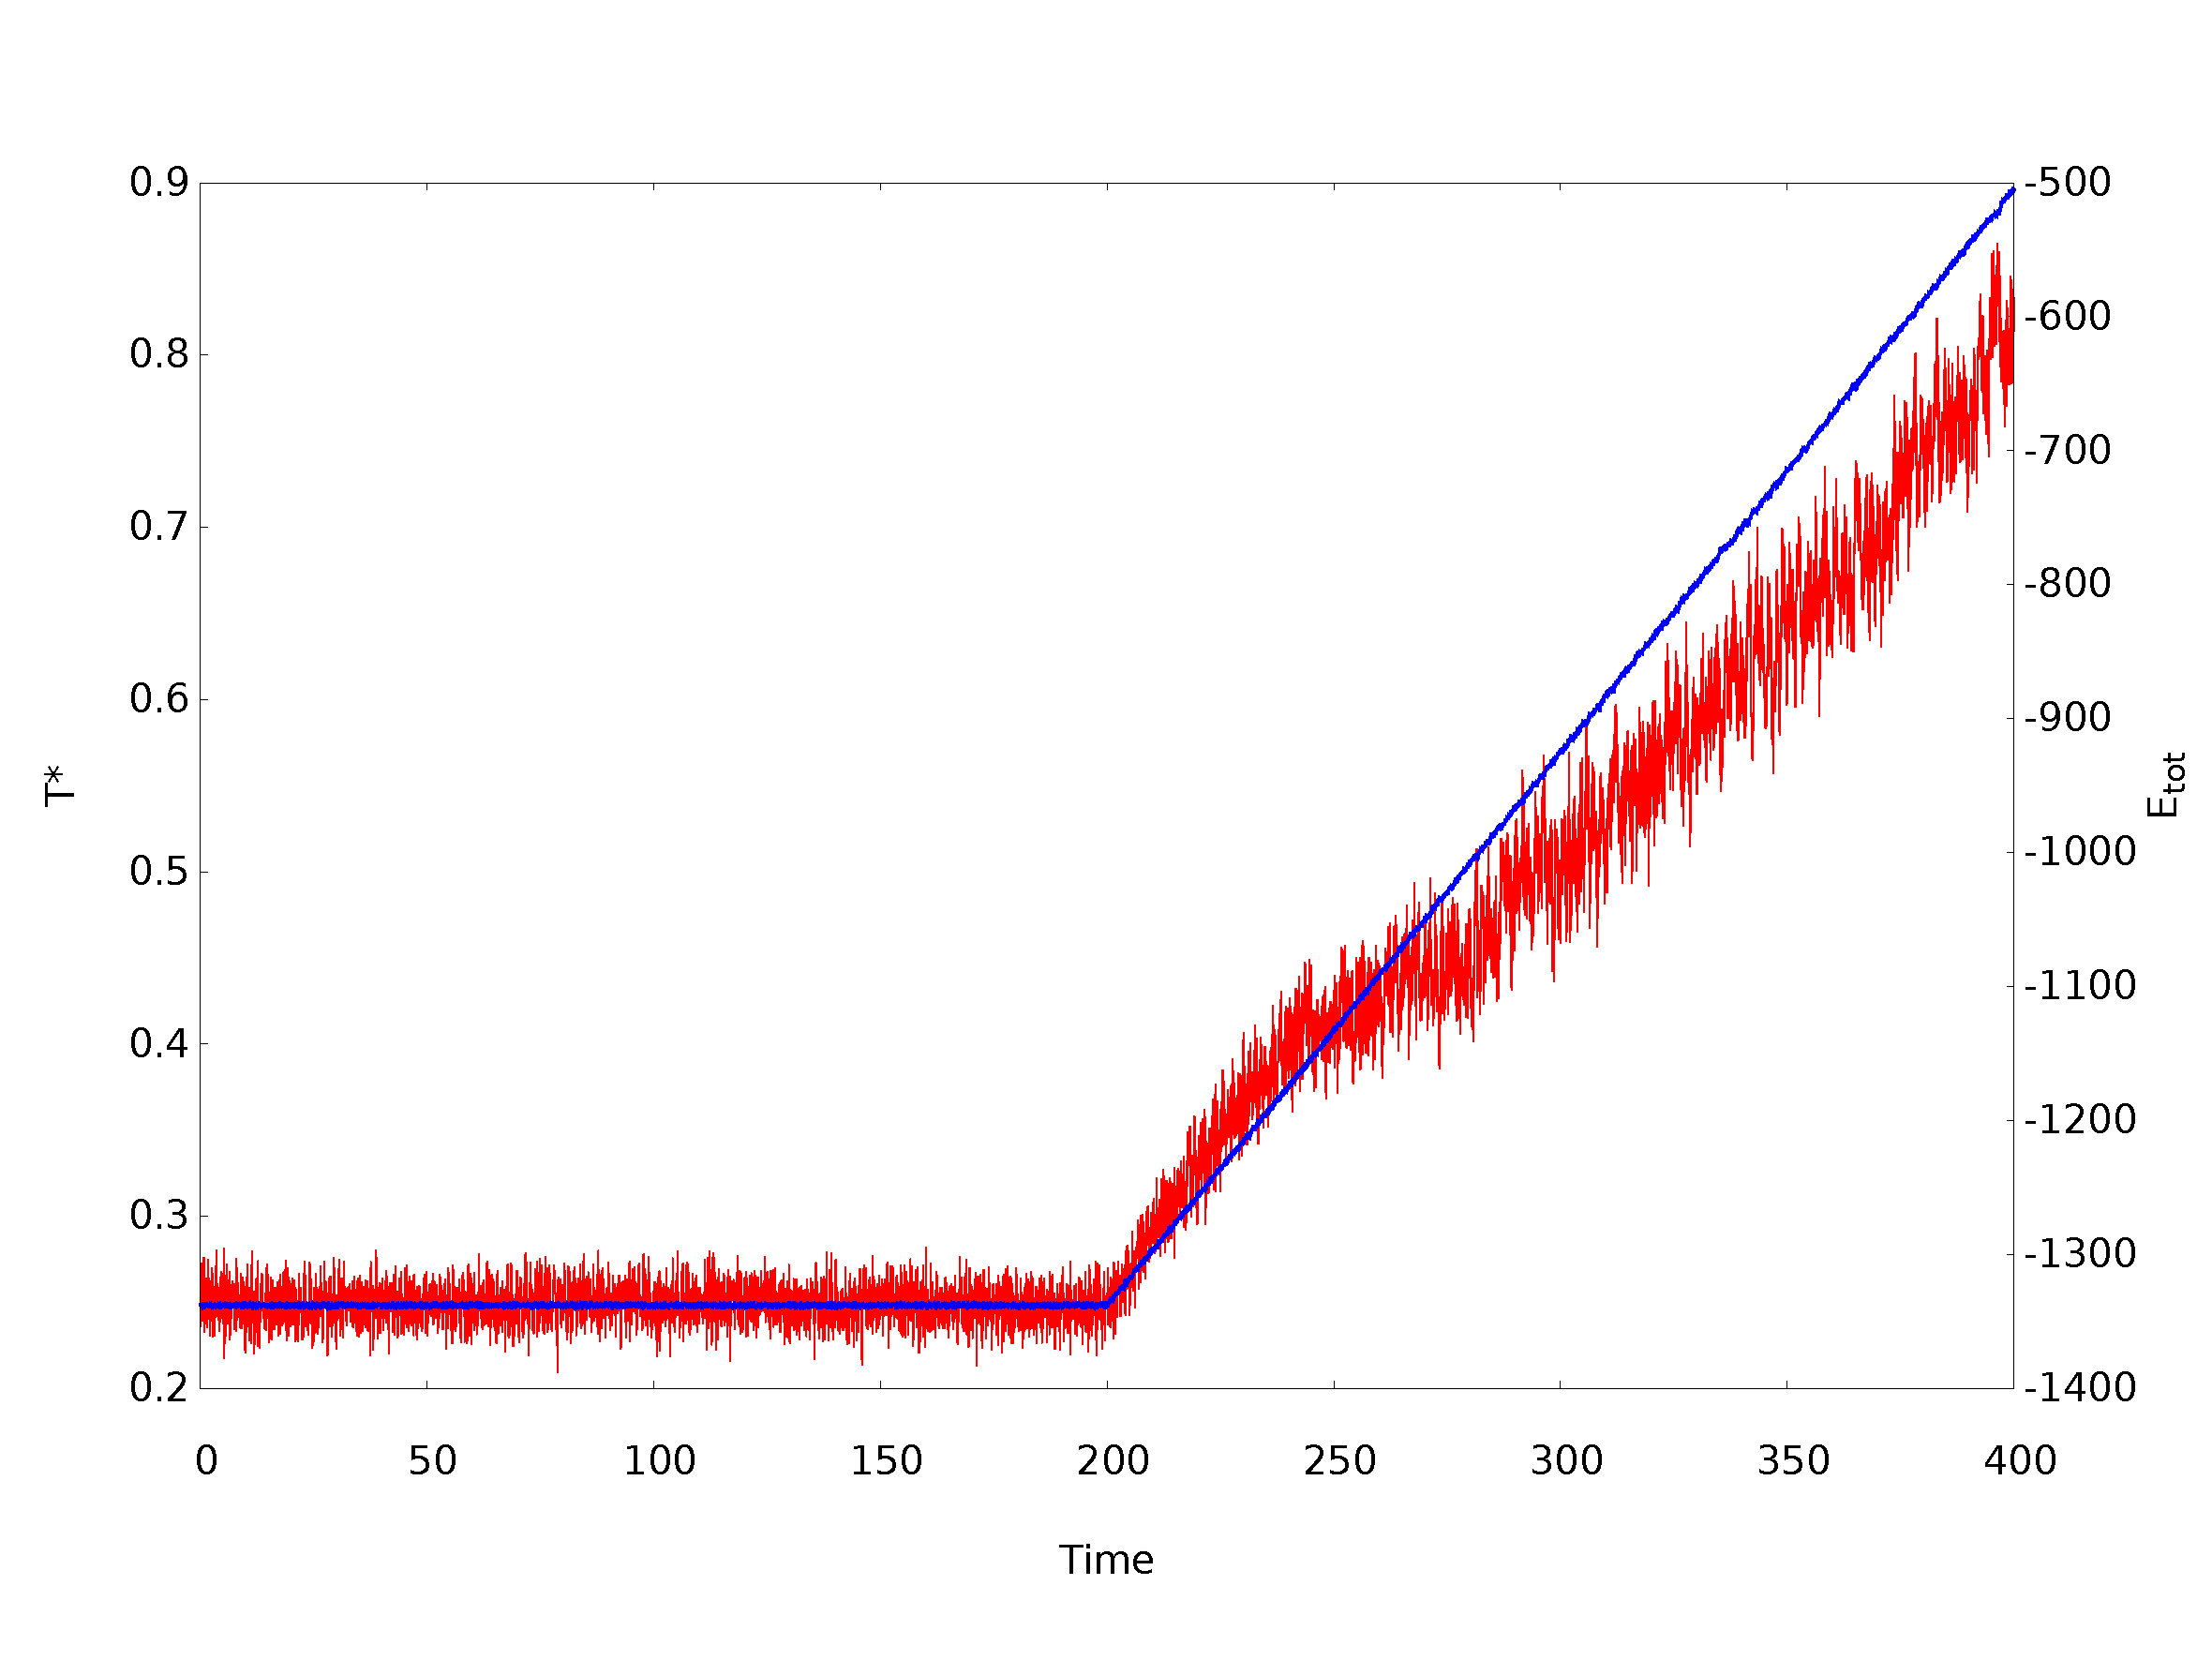
\includegraphics[scale=0.4]{images/ehex_te.pdf}
        \caption{Comparison of temperature (red) and energy (blue) during the application of the eHEX algorithm with $\Delta Q=0.04$ (in reduced units).
                The first 20000 timesteps, the energy and temperature are constant during the application of the velocity Verlet algorithm and start
            to rise, once the eHEX algortithm takes over. The values for the temperature can be seen on the ordinate on the left hand side
            and the values for the energy on the right hand side. }
        \label{fig:ehex_te}
    \end{center}
\end{figure}
The comparison of different values of $\Delta Q$ can be seen in Fig.~\ref{fig:ehex_dq}. As the correlation between the temperature and the energy has
been shown in Fig.~\ref{fig:ehex_te}, the plotting of the temperature data should suffice. 
\begin{figure}[h]
    \begin{center}
        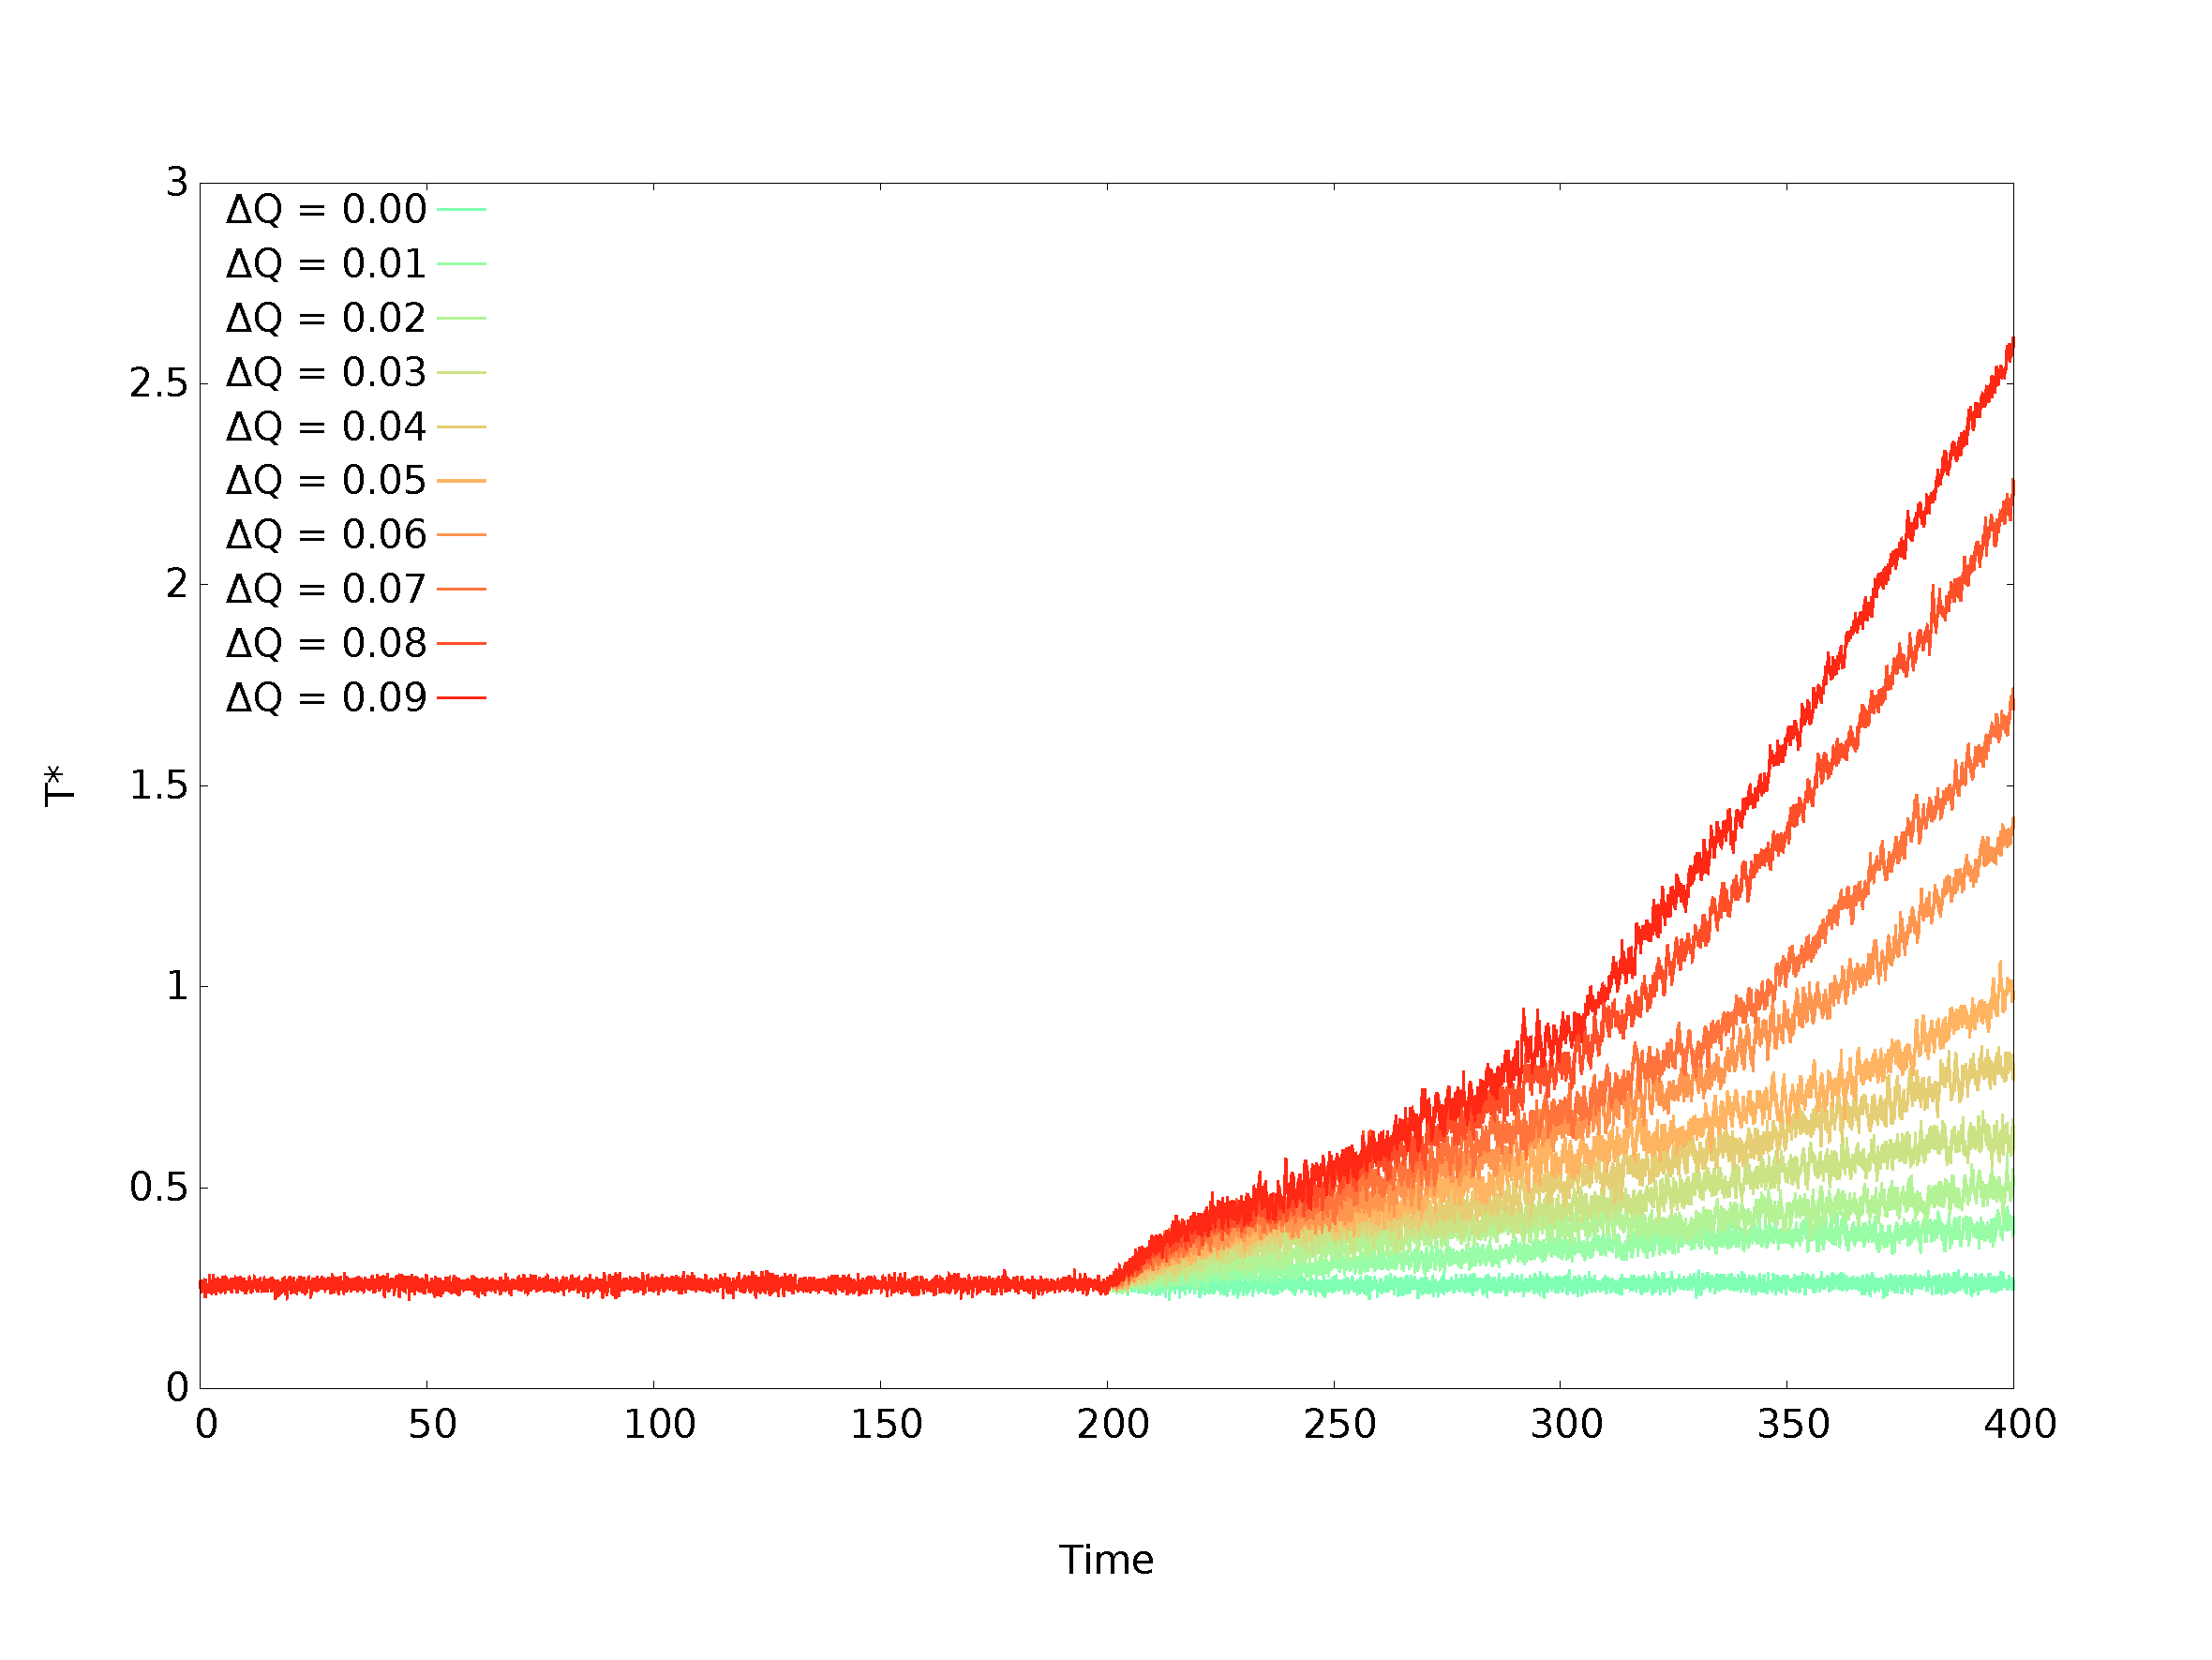
\includegraphics[scale=0.4]{images/ehex_temp_dq.pdf}
        \caption{Comparison of different values for $\Delta Q$, ranging from 0 to 0.09. As the value $\Delta Q=0$ corresponds to no heat being
        injected into the system, it is not surprising that the temperature remains constant. The graph shows that an increase in $\Delta Q$ leads to
    an increase in the rate of warming up, which means that for bigger $\Delta Q$, the system is heating up more quickly.}
        \label{fig:ehex_dq}
    \end{center}
\end{figure}

\subsection{Thermostat}
The barostat, as described previously, keeps the system from overheating. The barostat algorithm is applied at the same time as the eHEX algorithm,
after the velocity Verlet has equilibrated the system.\\
While the eHEX algorithm is pumping energy into the nano particle while the surrounding gas particles absorb excessive energy. This leads to the
development of a new, higher steady temperature of the nano particle, which can be seen in Fig.~\ref{fig:baro1}. 
%The first simulations were performed
%with the eHEX and the barostat algorithm starting at the same point. This lead to the question: does the new steady temperature depend on the time it
%takes the gas particles to reach the system? The answer is: no. After applying the barostat algorithm first to fill the box with gas atoms and then
%applying the eHEX algorithm it can be seen that the resulting temperature is the same, which can be seen in fig.~\ref{fig:baro2}.
%This means that the system is beginning to heat up, until the particles reach the crystal.
%Because of this, the temperature of the system rises, until it reaches a steady value again. This behaviour can be seen in fig.~\ref{fig:baro1}.\\
\begin{figure}[h]
    \begin{center}
        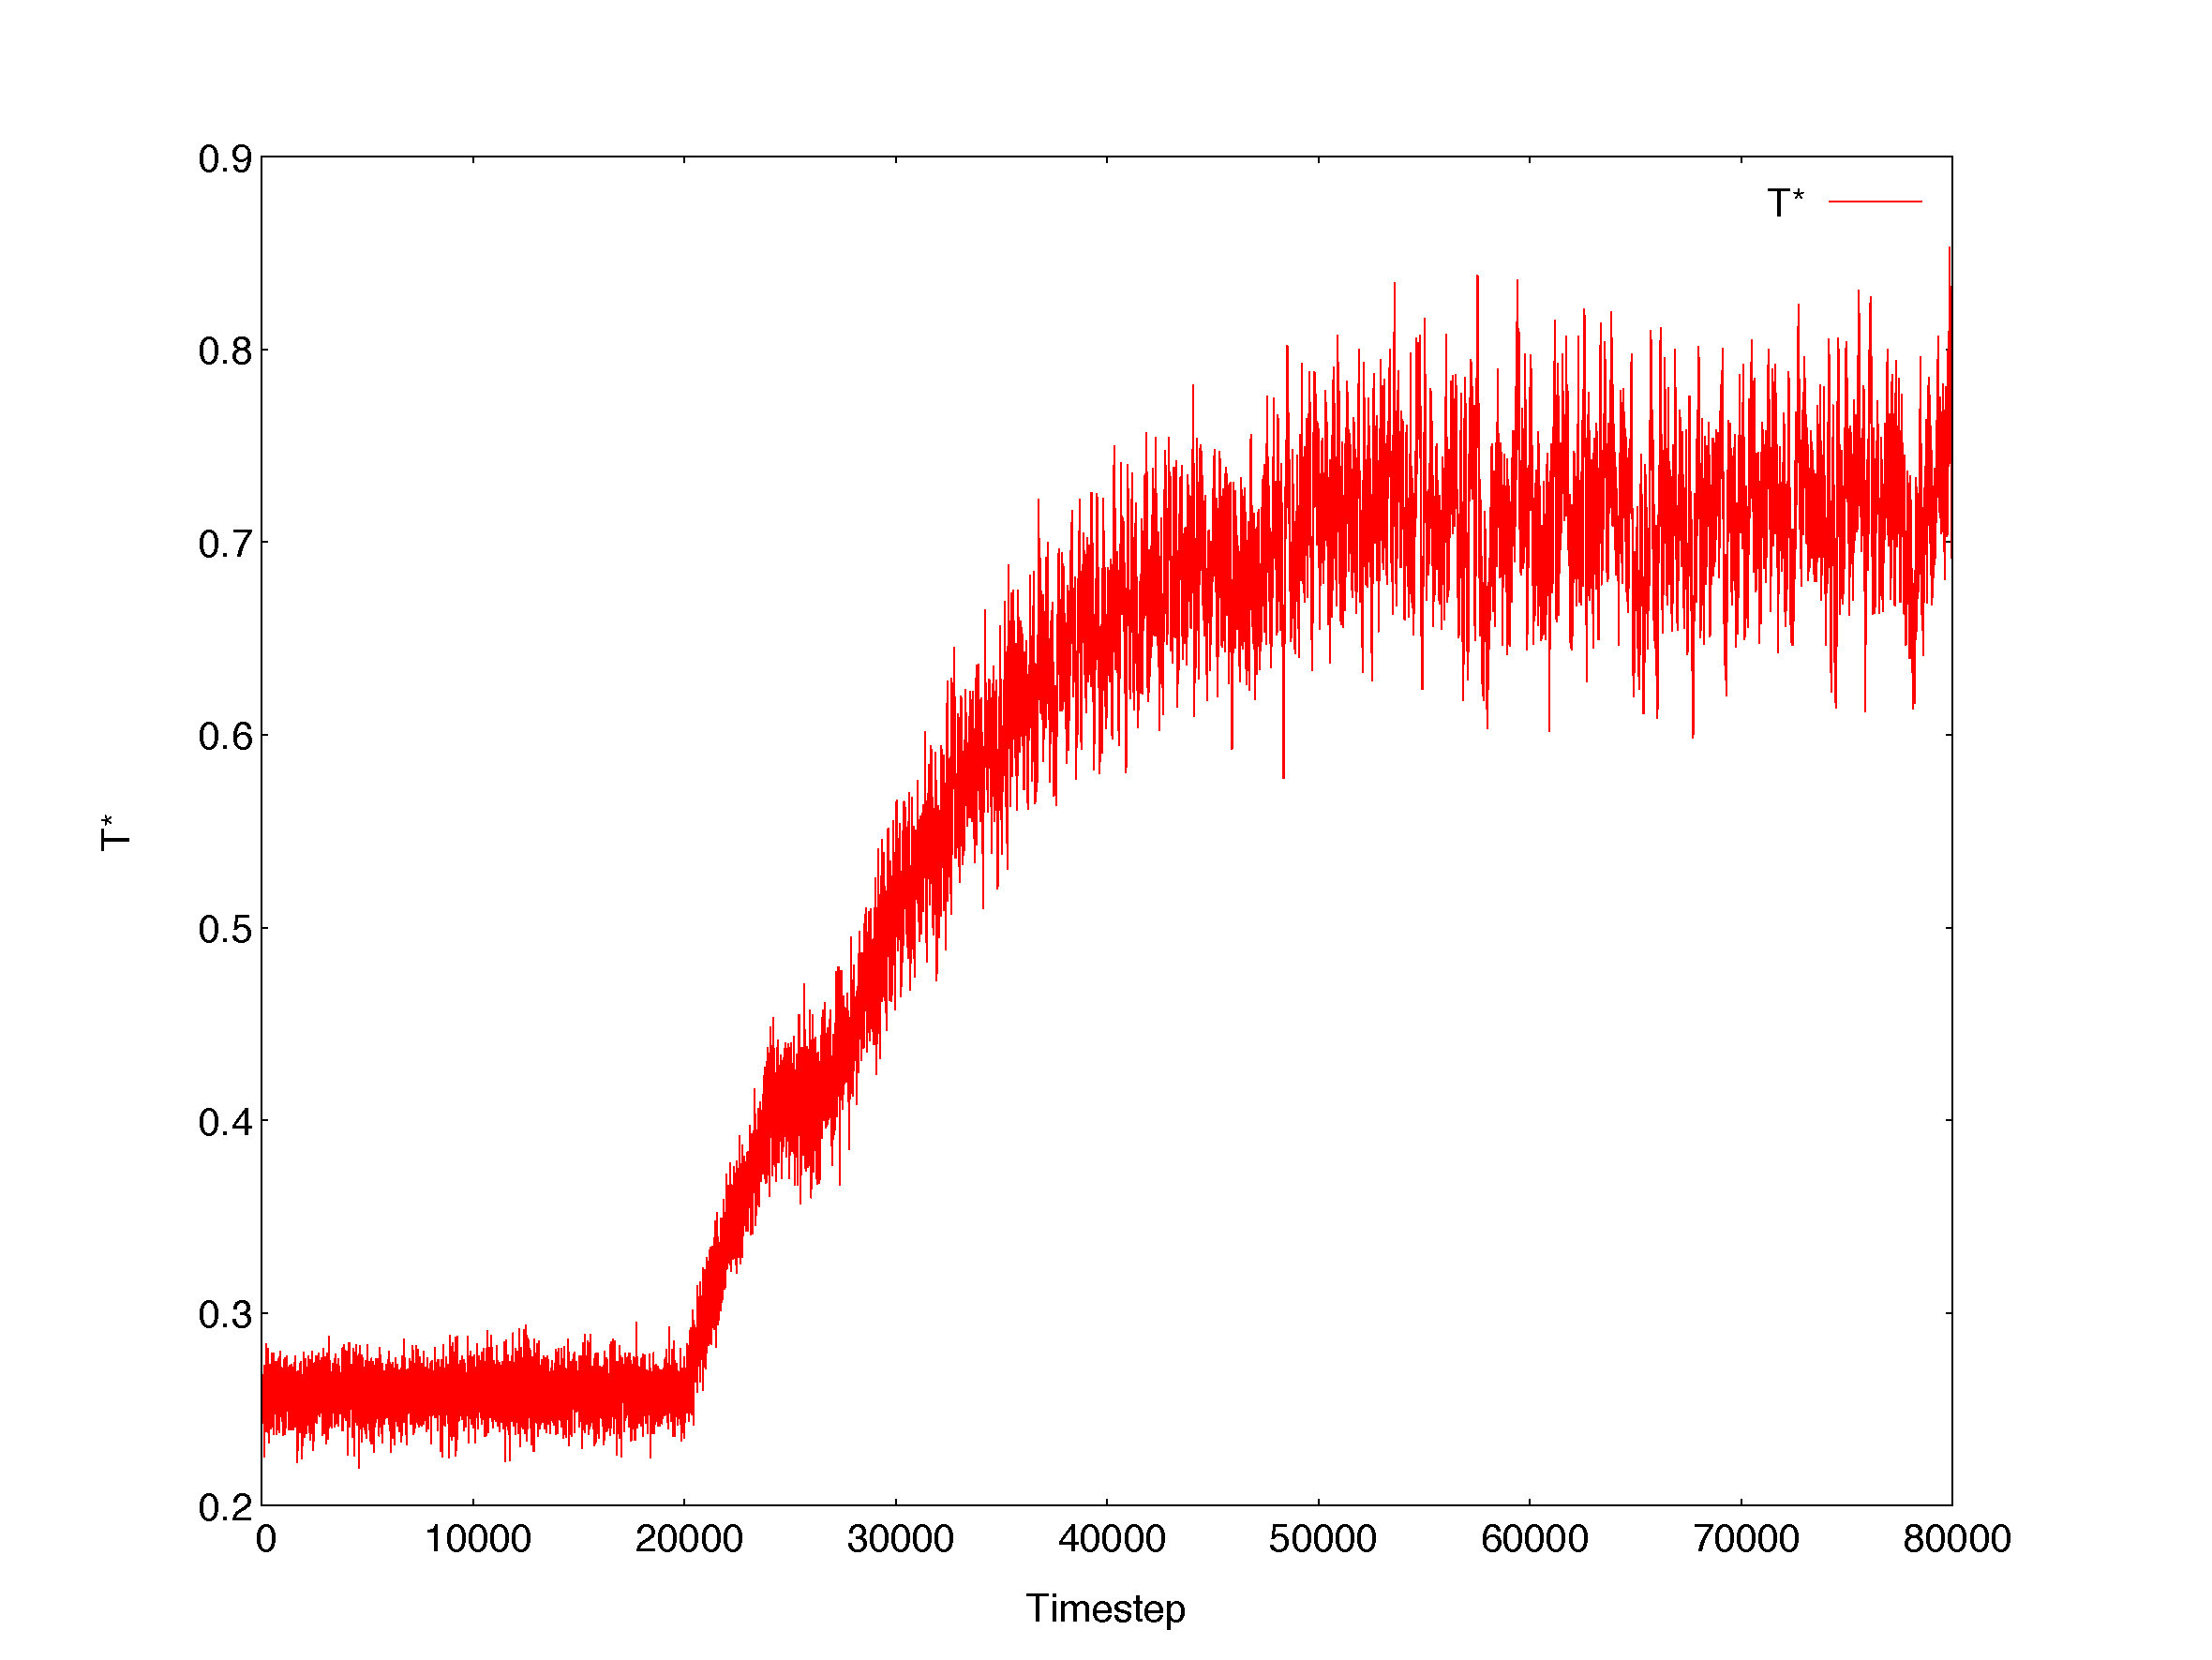
\includegraphics[scale=0.4]{images/baro_temp_start.pdf}
        \caption{Temperature of the system during the application of the eHEX and the barostat algorithm. During the first 20000 steps the system is
        in equilibrium while the velocity Verlet algorithm is applied. After that, the eHEX and the barostat algorithms are turned on. This leads to
    an increase in temperature until a new steady temperature is reached.}
        %\caption{Temperature of the system during the application of the eHEX and the barostat algorithm. During the first 20000 steps the system is
        %in equilibrium while the velocity Verlet algorithm is applied. After that, the eHEX and the barostat algorithms are turned on. This leads to
    %an increase in temperature until the gas particles reach the nano crystal to slow down the heating of the system. After some time, a plateau is
%reached and the temperature seems to stay at this value.}
        \label{fig:baro1}
    \end{center}
\end{figure}
%\begin{figure}[h]
    %\begin{center}
        %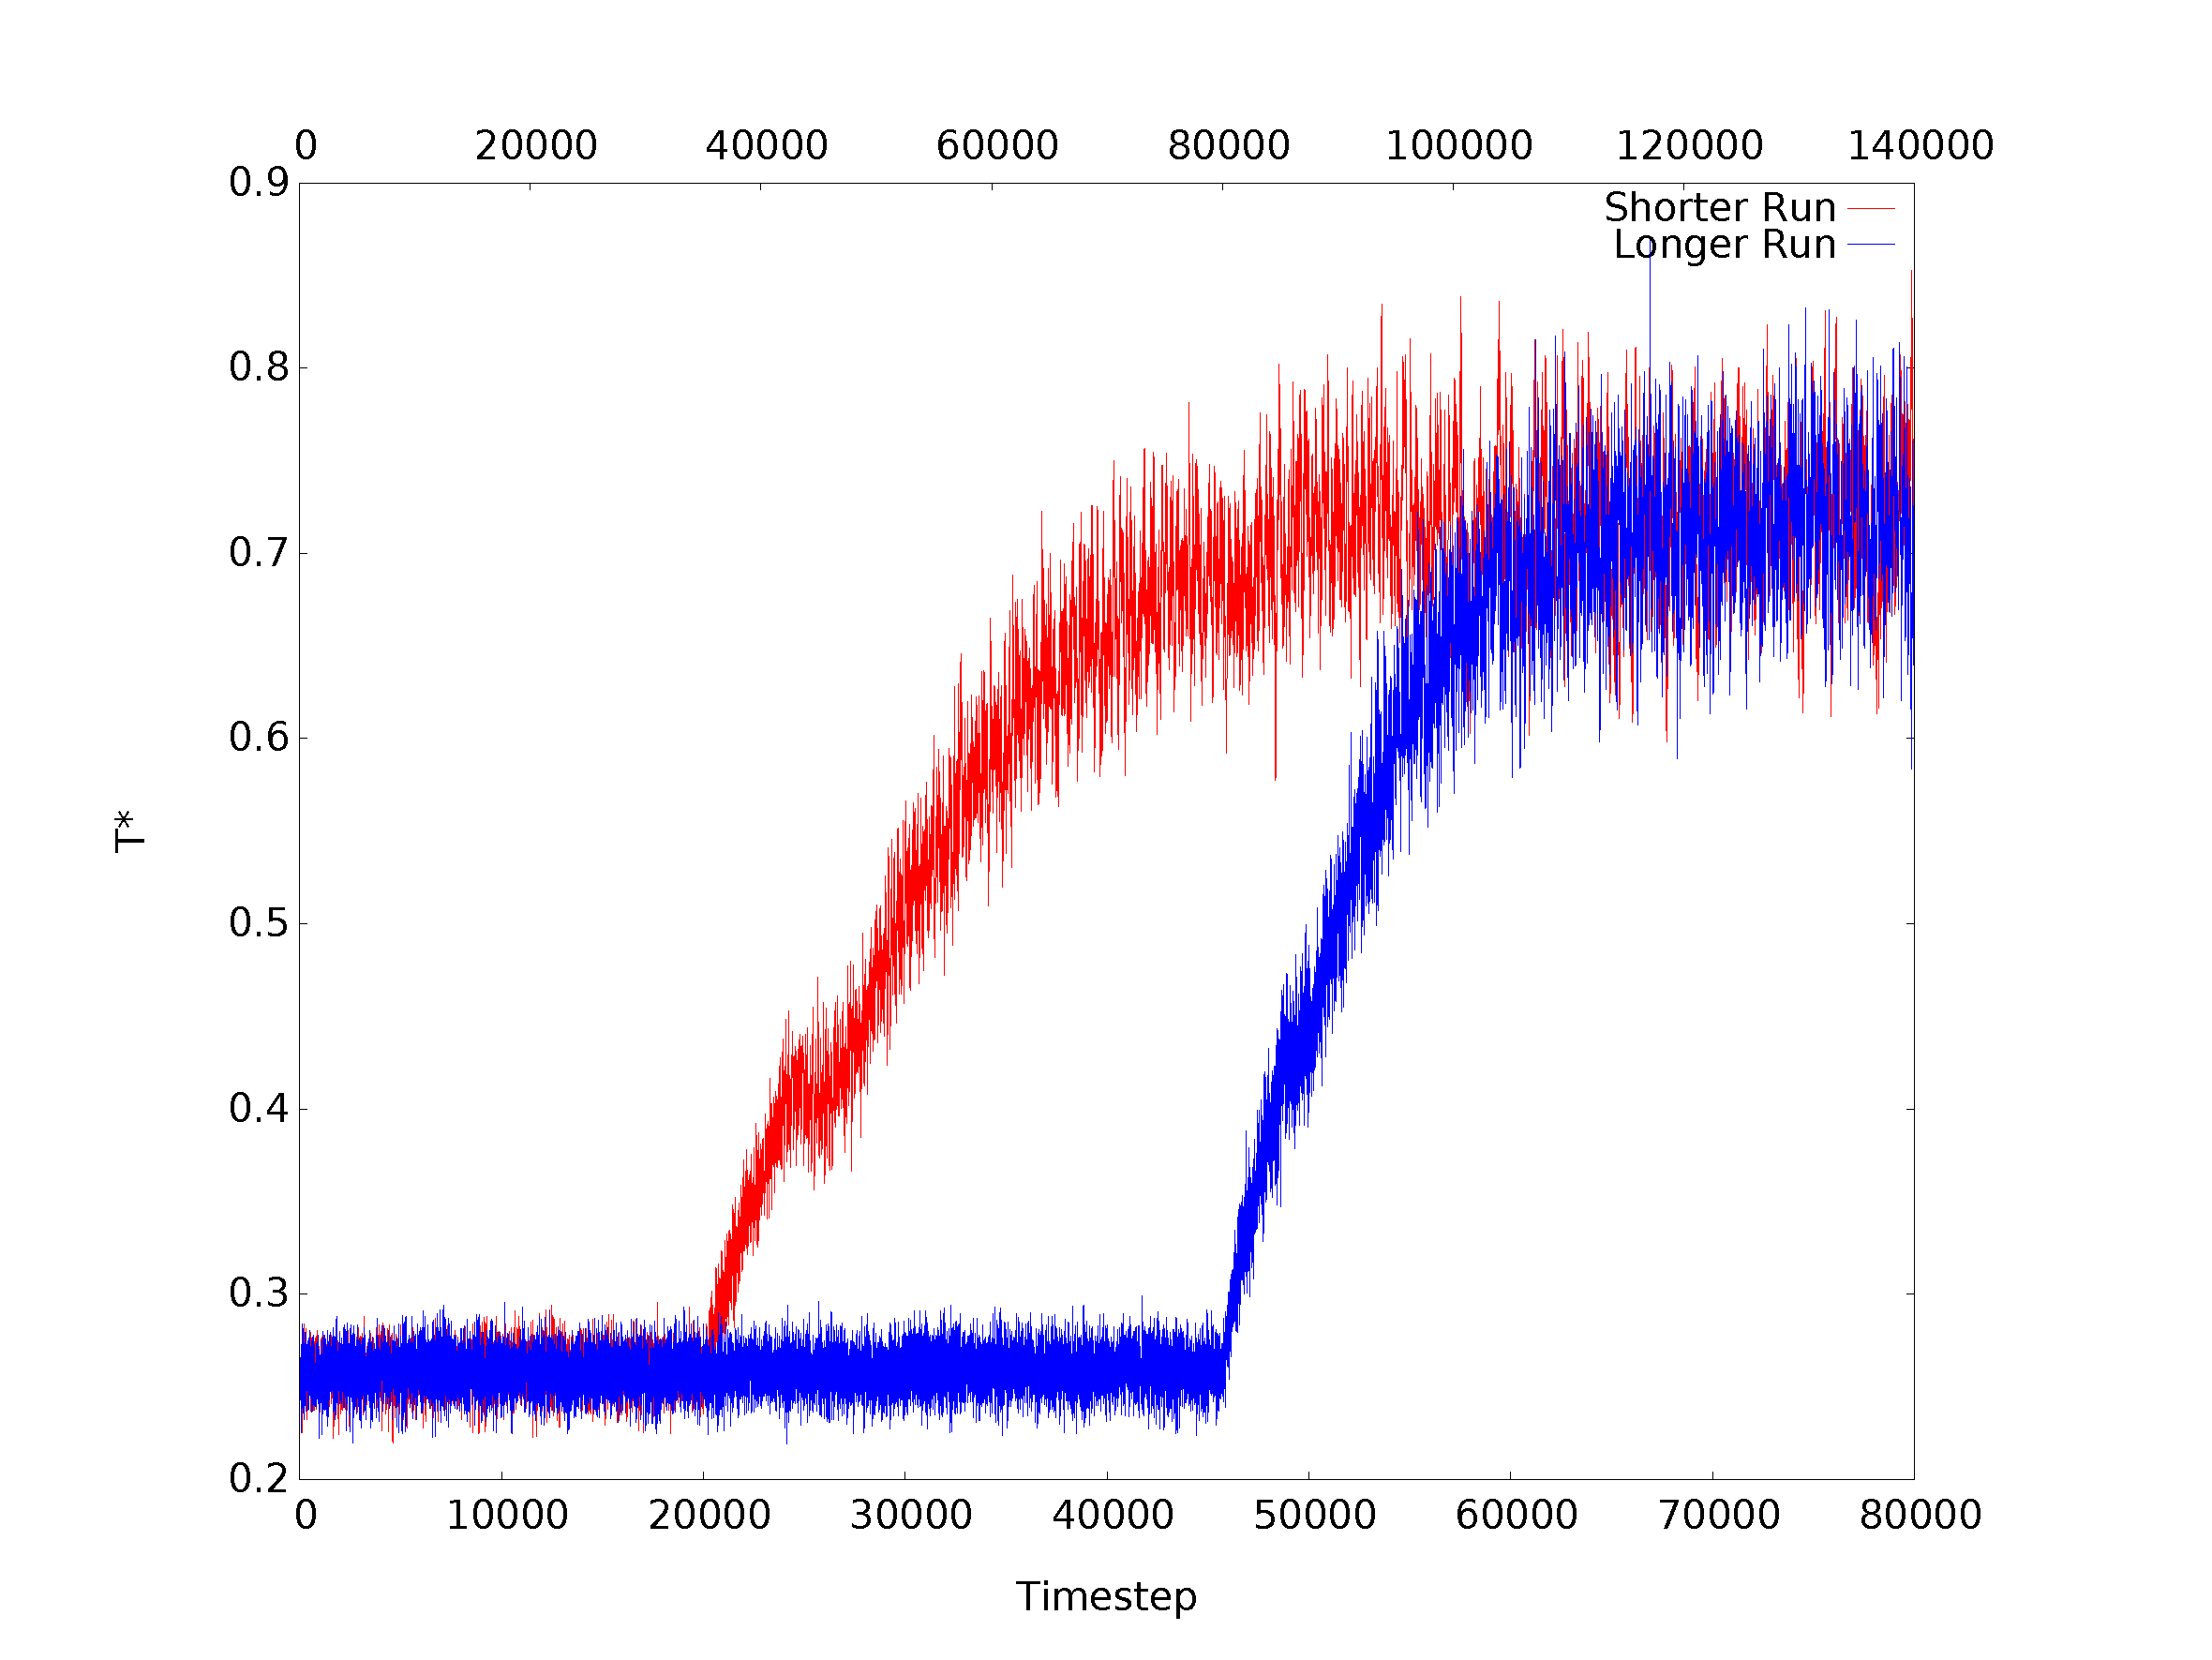
\includegraphics[scale=0.4]{images/baro_temp_compare_other.pdf}
        %\caption{Two versions of the application of the eEHX and barostat algorithm. The shorter run (red, x-axis on the bottom) represents 
            %the simultaneous start of the eHEX and the barostat algorithm. In the longer run (blue, x-axis on the top) there are 20000 steps, where
        %the barostat algorithm is applied at the same time as the velocity Verlet to give the system time to equilibrate and only after the eHEX
    %algorithm is taking the place of the velocity Verlet. The mean value of the resulting temperature is the same, indicating that the final
%temperature is based on the values of the parameters, such as pressure and ambient temperature, rather than geometry.}
        %%\caption{Temperature of the system during the application of the eHEX and the barostat algorithm. During the first 20000 steps the system is
        %%in equilibrium while the velocity Verlet algorithm is applied. After that, the eHEX and the barostat algorithms are turned on. This leads to
    %%an increase in temperature until the gas particles reach the nano crystal to slow down the heating of the system. After some time, a plateau is
%%reached and the temperature seems to stay at this value.}
        %\label{fig:baro1}
    %\end{center}
%\end{figure}
As we are interested in the temperatures of the particles before and after the interaction with the nano particle, we need some way to differentiate those
two states. This can be done when looking at the total energy of the gas particles.\\
The gas particles are created on the surface of the simulation box, which is further away than the interaction range between the gas particles and the
nano particle. Since the gas particles do not interact with each other, the total energy of the gas particles does not change until they reach the
interaction range of the nano particle. There they undergo a change of energy due to the interaction with the nano particle and then make their way away
from the nano particle. After the interaction, when they reach a point outside of the interaction range, the enrgy stays constant again until the
particles reach the limits of the simulation box.\\
Therefore, the life span of a single gas particle can be partioned into 3 stages: incoming, interacting, outgoing. In a typical scene of interaction
all three of these stages are represented by different gas particles, as can be seen in Fig.~\ref{fig:barointeraction}.\\
\begin{figure}[h]
    \begin{center}
        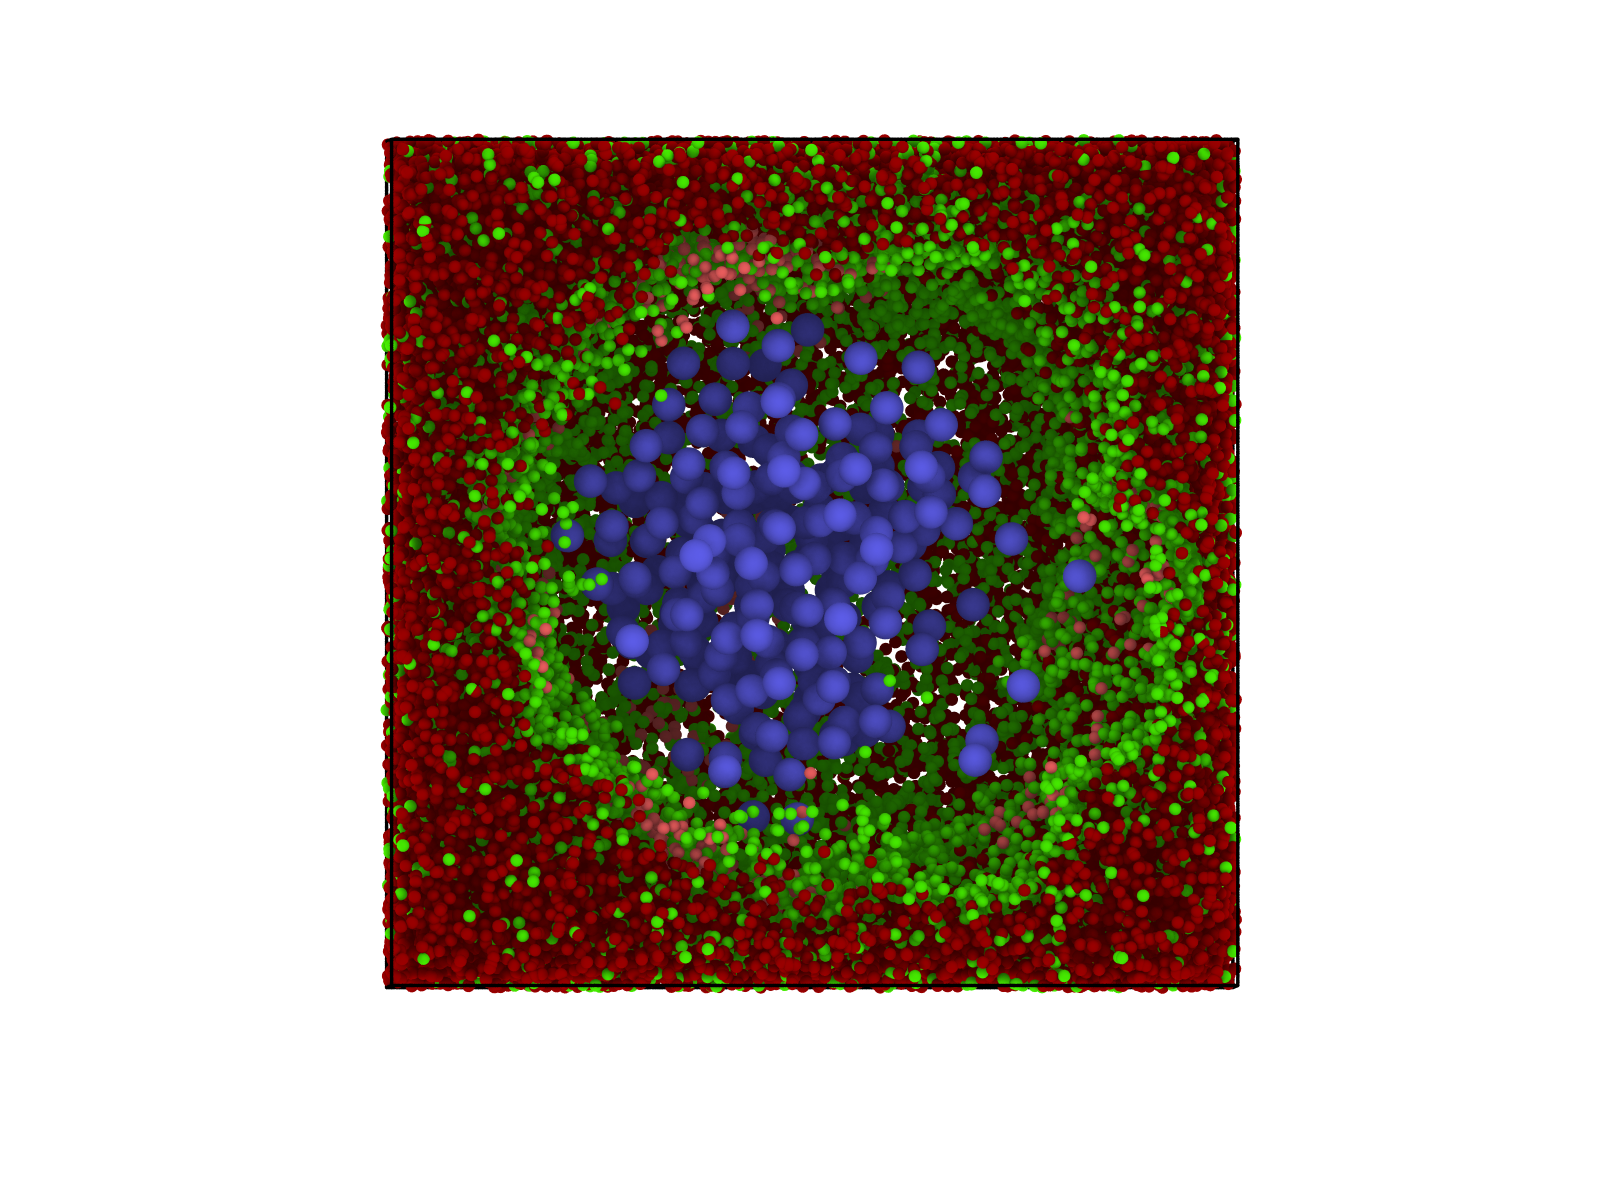
\includegraphics[scale=0.4]{images/baro_170105_new_medium.png}
        \caption{Rendering of the application of the barostat algorithm. The red particles are incoming gas particles, that have not yet interacted, 
            pink particles are currently interacting and green particles are leaving the simulation box and
        moving away from the nano particle (blue). To render this image, a cut has been made to make a view into the simulation box possible.}
        \label{fig:barointeraction}
    \end{center}
\end{figure}
Since the gas particles are interacting with the nano particle, the temperatures and energies are values of interest. The energies are recorded using
histograms and the temperature is calculated instantaneously every 100th timestep.\\
The calculation of the energies of the incoming particles has to be done with care. The problem are particles that enter the simulation box, but fly
by the nano particle at a distance that is greater than the interaction range. Since the change of the energy is the interesting part, only the energy 
particles of that \textit{do} interact with the nano particle shall be calculated. This can be achieved by counting particles that enter the stage of
\textit{interacing}. One such histogram can be seen in Fig.~\ref{fig:histogram}.
\begin{figure}[h]
    \begin{center}
        \includegraphics[scale=0.4]{images/histogram_2.pdf}
        \caption{Histogram of total energies for incoming (red) and outgoing (blue) particles. The parameters for this histogram are $\Delta Q^*=0.04$,
        $T_\text{ambient}^*=0.08$, $P^*=0.8$. What can be seen here is that the outgoing particles have a higher count of particles with more total
    energy.}
        \label{fig:histogram}
    \end{center}
\end{figure}





%\begin{figure}[h]
    %\begin{center}
        %\begin{subfigure}[t]{0.3\textwidth}
            %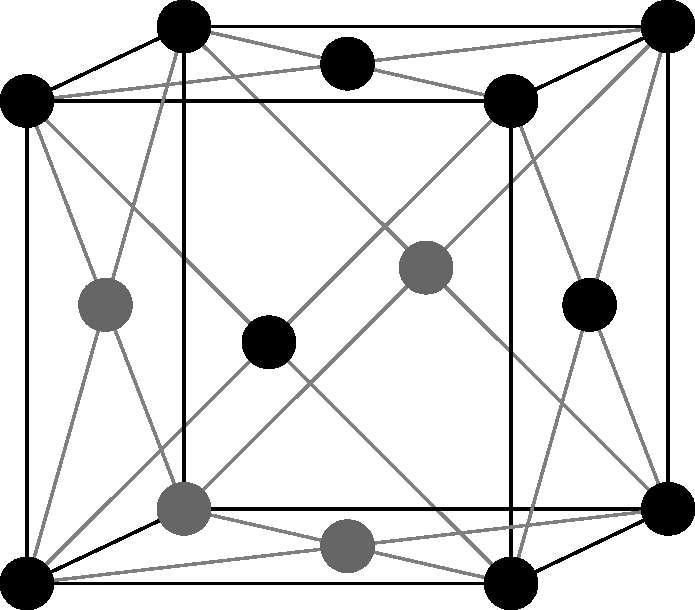
\includegraphics[scale=0.3]{images/fcc-2.pdf}
            %\caption{Schematic figure of a face centered cubic (FCC) lattice}
            %\label{fig:fcc}
        %\end{subfigure} 
        %\
        %\begin{subfigure}[t]{0.3\textwidth}
            %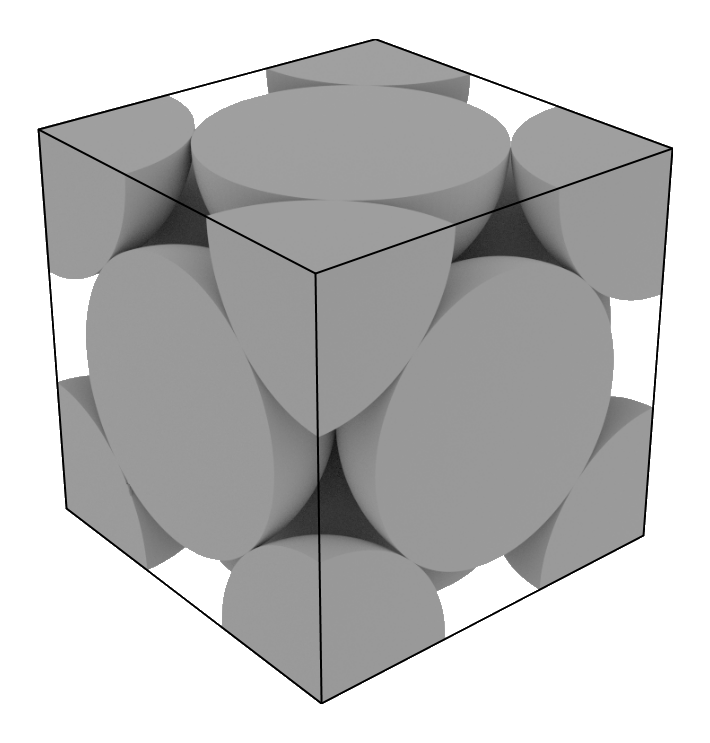
\includegraphics[scale=0.15]{images/fcc_unit.png}
            %\caption{Schematic of the number of particles contained in one FCC unit cell. The atoms on the edges are shared by 8 cells and the ones 
                %on the faces by 2 cells\cite{unitcell}}
            %\label{fig:fcccut}
        %\end{subfigure} 
        %\
        %%\hspace{60pt}
        %\begin{subfigure}[t]{0.3\textwidth}
            %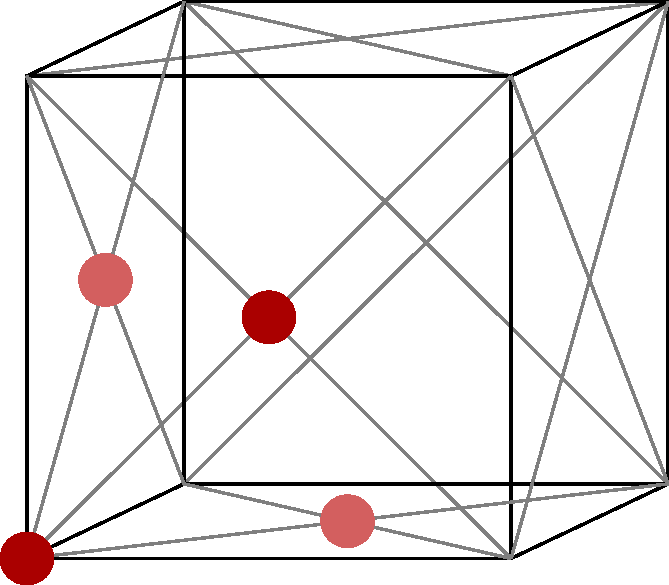
\includegraphics[scale=0.3]{images/unit_cell.pdf}
            %\caption{Setup for successively building a FCC lattice}
            %\label{fig:unitcell}
        %\end{subfigure}
    %\end{center}
%\end{figure}



\newpage
\section{Conclusion}
% what does this all tell us? do we need to study more of this? 






\newpage
\bibliography{references}
\bibliographystyle{unsrt}

\end{document}
